\fontsize{13pt}{22.5pt}\selectfont

\section{THIẾT KẾ MÔI TRƯỜNG VÀ PHƯƠNG PHÁP THỰC NGHIỆM}
\label{ch:design}

\indent Chương này thuật lại quá trình biến ý tưởng của đề tài thành một hệ thống thực
nghiệm chạy được. Phần đầu chương dành cho những gì áp dụng chung cho cả ba môi trường:
kiến trúc huấn luyện, cách chọn quan sát và hành động, và bốn nguyên tắc thiết kế hàm
phần thưởng mà mọi con số trong các bảng về sau đều phải giải thích được bằng chúng. Ba
mục kế tiếp đi vào từng môi trường một. Chương khép lại bằng lối đi vòng qua Python
Low-Level API - thứ mà đề tài buộc phải dùng đến vì trainer tích hợp sẵn không đáp ứng
được - rồi tới thiết lập thực nghiệm và tiêu chí đánh giá.

% ═══════════════════════════════════════════════
\subsection{Tổng quan thiết kế hệ thống}

\subsubsection{Kiến trúc huấn luyện tổng thể}
\indent Toàn bộ hệ thống thực nghiệm được xây dựng theo kiến trúc client-server của
Unity ML-Agents đã trình bày ở Mục~\ref{sub:mlarch}. Trong kiến trúc này, Unity đảm
nhận vai trò mô phỏng: nó dựng nên thế giới ba chiều, tính toán vật lý va chạm, thu
thập quan sát của tác nhân và thực thi các hành động mà tác nhân lựa chọn. Phía Python,
thông qua chương trình \texttt{mlagents-learn}, đảm nhận vai trò huấn luyện: nó nhận
quan sát từ Unity, suy luận ra hành động dựa trên chính sách hiện tại và cập nhật tham
số của mạng nơ-ron dựa trên phần thưởng thu về. Hai phía trao đổi dữ liệu với nhau
theo từng bước thời gian thông qua giao thức truyền thông nội bộ.

{\sloppy
\indent Ba môi trường của đề tài được tổ chức thành ba khu vực độc lập trong cùng một
dự án Unity, tương ứng với ba thư mục \texttt{Assets/\allowbreak Football},
\texttt{Assets/\allowbreak Collaboration} và \texttt{Assets/\allowbreak CrossTheRoad}.
Mỗi môi trường được gắn
với một loại hành vi riêng, lần lượt mang tên \texttt{Football}, \texttt{PuzzleBehavior}
và \texttt{CrossTheRoad}. Việc tách biệt này cho phép huấn luyện từng môi trường một
cách độc lập mà không gây nhiễu lẫn nhau, đồng thời giúp việc nạp đúng tệp cấu hình
cho từng lần chạy trở nên rõ ràng.\par}

\indent Ở mỗi môi trường, toàn bộ nội dung của một lượt chơi được gom vào một khu vực
huấn luyện và đóng gói thành một prefab độc lập. Cách tổ chức này cho phép nhân bản
khu vực thành nhiều bản sao đặt cạnh nhau trong cùng một cảnh để thu thập nhiều mẫu
kinh nghiệm cùng lúc; trong các lần huấn luyện được báo cáo ở Chương~\ref{ch:results},
mỗi cảnh chỉ chứa đúng một khu vực, nên tốc độ thu thập dữ liệu hoàn toàn đến từ hệ số
tăng tốc mô phỏng. Hệ số này được đặt ở mức gấp hai mươi lần thời gian thực, cho phép
Unity mô phỏng nhanh hơn nhiều so với tốc độ hiển thị thông thường mà không ảnh hưởng
đến tính đúng đắn của vật lý. Toàn bộ chín lần huấn luyện của đề tài được điều phối tự
động bằng một chương trình Python trình bày ở Mục~\ref{sub:codestruct}.

\subsubsection{Không gian quan sát}
\label{sub:obs-space}
\indent Trong một hệ thống học tăng cường, cần phân biệt rành mạch giữa trạng
thái của môi trường và quan sát mà tác nhân nhận được. Trạng thái là toàn bộ
lượng thông tin mô tả đầy đủ tình huống hiện tại của thế giới mô phỏng, bao gồm cả
những đại lượng mà tác nhân không thể trực tiếp cảm nhận; trong khi đó quan sát chỉ là
phần thông tin mà tác nhân thực sự tiếp cận được thông qua các cảm biến của nó. Sự phân
biệt này là điểm xuất phát cho mọi quyết định thiết kế về sau, vì thế trước hết đề tài
phát biểu nó một cách hình thức.

\begin{dn}[Không gian quan sát]
\label{dn:obs}
Cho môi trường có không gian trạng thái $S$. Không gian quan sát $\Omega$ là tập hợp
tất cả các quan sát khả dĩ mà tác nhân có thể nhận được. Hàm quan sát
$O: S \to \Omega$ ánh xạ mỗi trạng thái $s \in S$ sang một quan sát $o = O(s)$ mà tác
nhân dùng làm căn cứ duy nhất để ra quyết định tại bước thời gian tương ứng.
\end{dn}

\indent Khi hàm quan sát $O$ là song ánh, mỗi quan sát tương ứng với đúng một trạng
thái, và tác nhân có thể coi như ``nhìn thấy'' toàn bộ trạng thái; bài toán khi đó là
một quá trình quyết định Markov (MDP) đầy đủ như đã trình bày ở Mục~\ref{sub:mdp}.
Ngược lại, khi $O$ không song ánh, tức khi nhiều trạng thái khác nhau cùng cho ra một
quan sát, tác nhân không thể phân biệt các trạng thái đó và bài toán trở thành một
quá trình quyết định Markov quan sát một phần (Partially Observable MDP, viết
tắt POMDP). Phần lớn các môi trường trong game, kể cả ba môi trường của đề tài, về bản
chất là POMDP: một tác nhân không thể biết chính xác vận tốc tương lai của một phương
tiện, cũng như không thể nhìn xuyên qua tường để biết vị trí đồng đội. Nhiệm vụ của
người thiết kế, do đó, không phải là cung cấp toàn bộ trạng thái, mà là chọn ra một
tập quan sát đủ để bài toán xấp xỉ được tính chất Markov, tức là để quan sát
hiện tại một mình đã chứa gần như toàn bộ thông tin cần thiết cho một quyết định hợp
lý, mà không buộc tác nhân phải ghi nhớ toàn bộ lịch sử.

\begin{dn}[Tính chất Markov của quan sát]
\label{dn:markov-obs}
Một biểu diễn quan sát được gọi là thỏa mãn tính chất Markov nếu phân phối xác suất
của trạng thái kế tiếp và phần thưởng chỉ phụ thuộc vào quan sát và hành động hiện tại,
mà không phụ thuộc thêm vào bất kỳ quan sát nào trong quá khứ:
\[
\Pr\bigl(o_{t+1}, r_{t+1} \mid o_t, a_t, o_{t-1}, a_{t-1}, \dots\bigr)
= \Pr\bigl(o_{t+1}, r_{t+1} \mid o_t, a_t\bigr).
\]
\end{dn}

\indent Trong thực tế, hiếm khi đạt được tính chất Markov một cách tuyệt đối, nên mục
tiêu thiết kế là làm cho nó gần đúng nhất có thể với chi phí quan sát thấp nhất.
Có hai kỹ thuật bổ trợ thường dùng khi một quan sát tức thời chưa đủ Markov. Kỹ thuật
chồng khung ghép nối một số quan sát liên tiếp gần nhất thành một vector duy
nhất, nhờ đó thông tin về xu hướng chuyển động, chẳng hạn vận tốc suy ra từ hiệu vị trí
giữa hai khung, được đưa vào tường minh. Cách còn lại là dùng mạng có bộ nhớ hồi tiếp để
tác nhân tự tổng hợp lịch sử. Đề tài chủ yếu dùng chồng khung và bổ sung trực tiếp các
đại lượng động như vận tốc vào vector quan sát, nhằm giữ cho mạng chính sách đơn giản và
ổn định.

\indent Cả ba môi trường của đề tài đều dùng dạng quan sát vector, tức một chuỗi
số thực có độ dài cố định, trong đó mỗi phần tử mã hóa một đại lượng có ý nghĩa vật lý
hoặc logic. Ba loại đại lượng thường gặp gồm các đại lượng liên tục như tọa độ, vận
tốc, khoảng cách hay góc xoay; các cờ nhị phân biểu diễn trạng thái logic, chẳng hạn một
bàn đạp đã được nhấn hay chưa, được mã hóa bằng giá trị không hoặc một; và mã hóa
một-nóng dùng khi cần biểu diễn một biến rời rạc có nhiều mức. Nguyên tắc xuyên suốt là chỉ đưa vào những đại lượng
tối thiểu nhưng đủ; mỗi phần tử thừa đều làm tăng số chiều đầu vào của mạng và khiến
việc học chậm hơn, trong khi mỗi phần tử thiếu có thể phá vỡ tính chất Markov và khiến
bài toán trở nên bất khả học.

\indent Để quá trình huấn luyện ổn định, các giá trị quan sát liên tục được
chuẩn hóa về lân cận khoảng $[-1, 1]$ trước khi đưa vào mạng nơ-ron. Với một
đại lượng $x$ có kỳ vọng $\mu$ và độ lệch chuẩn $\sigma$ ước lượng trực tuyến trong
quá trình chạy, giá trị chuẩn hóa là $\hat{x} = (x - \mu)/\sigma$. Việc chuẩn hóa đặc
biệt thiết yếu với môi trường Football Table, nơi các đại lượng như vận tốc bóng và
góc xoay thanh gạt có thang đo chênh nhau nhiều bậc; nếu để nguyên, những đại lượng
giá trị lớn sẽ tạo ra gradient lấn át và làm sai lệch việc học của các đại lượng nhỏ.

\indent Bên cạnh quan sát vector, hai môi trường Cross The Road và Capture The Flag
còn được trang bị cảm biến tia, một cơ chế quan sát không gian mô phỏng thị
giác của thực thể trong thế giới ba chiều. Cảm biến phóng ra một chùm gồm nhiều tia từ
vị trí tác nhân, trải đều trong một góc quạt phía trước. Mỗi tia dò tìm vật thể đầu
tiên mà nó chạm tới trong một tầm xa giới hạn, rồi trả về hai loại thông tin: một là
loại vật thể bị chạm, mã hóa một-nóng trên tập các nhãn cần phát hiện, hai là khoảng
cách chuẩn hóa từ tác nhân tới điểm chạm. Nếu gọi $k$ là số tia và $m$ là số nhãn vật
thể cần phát hiện, thì mỗi tia sinh ra $m + 2$ giá trị, gồm $m$ giá trị một-nóng cho
nhãn, một giá trị báo tia có chạm gì không, và một giá trị khoảng cách; tổng số chiều
quan sát do cảm biến tia đóng góp là $k \times (m + 2)$. Nhờ cảm biến này, một tác nhân
trong môi trường Capture The Flag có thể phát hiện được tường, cửa, bàn đạp, điểm đích
và cả đồng đội ở trong tầm nhìn, mà không cần được cung cấp tọa độ tuyệt đối của chúng.

\subsubsection{Không gian hành động}
\label{sub:action-space}
\indent Tương ứng với quan sát ở đầu vào, hành động là đầu ra mà chính sách của tác
nhân sinh ra ở mỗi bước để tác động lên môi trường.

\begin{dn}[Không gian hành động]
\label{dn:action}
Không gian hành động $A$ là tập hợp tất cả các hành động mà tác nhân được phép thực
hiện. Không gian này được gọi là rời rạc nếu $A$ là một tập hữu hạn các lựa
chọn, và được gọi là liên tục nếu $A$ là một tập con của không gian số thực
nhiều chiều $\mathbb{R}^{n}$, khi đó mỗi hành động là một vector số thực bị chặn trong
một khoảng cho trước.
\end{dn}

\indent Sự khác nhau giữa hai dạng không gian hành động dẫn tới hai cách mà mạng chính
sách biểu diễn đầu ra. Với không gian rời rạc, mạng xuất ra một phân phối xác suất trên
tập hành động và tác nhân lấy mẫu một hành động từ phân phối đó; trường hợp có nhiều
nhóm hành động độc lập, ML-Agents dùng dạng đa rời rạc, trong
đó mỗi nhóm là một nhánh có phân phối riêng. Với không gian liên tục, mạng thường xuất
ra các tham số của một phân phối chuẩn nhiều chiều, gồm kỳ vọng và độ lệch chuẩn cho
mỗi chiều, rồi hành động được lấy mẫu và cắt về khoảng hợp lệ. Chính vì cách biểu diễn
khác nhau này mà một số thuật toán tỏ ra phù hợp hơn với một dạng không gian nhất định;
đặc biệt, SAC được thiết kế nguyên thủy cho điều khiển liên tục và phát huy thế mạnh
rõ nhất ở đó.

\indent Đề tài chủ ý lựa chọn ba môi trường phủ cả hai dạng không gian hành động nhằm
đánh giá tính linh hoạt của từng thuật toán. Môi trường Football Table dùng không gian
hành động liên tục tám chiều: bốn thanh gạt, mỗi thanh gồm một chiều điều khiển
lực trượt ngang và một chiều điều khiển lực xoay, mỗi chiều nhận một giá trị thực phản
ánh bản chất điều khiển vật lý mượt mà của trò chơi bi lắc. Hai môi trường còn lại dùng
không gian hành động rời rạc một nhánh. Cross The Road có bốn hành động gồm đứng
yên, sang trái, sang phải và tiến; Capture The Flag có bảy hành động gồm đứng yên,
tiến, lùi, xoay trái, xoay phải, đi ngang sang trái và đi ngang sang phải. Một điểm cần
nhấn mạnh là quan hệ giữa hành động được chọn và chuyển động thực tế của tác nhân, vốn
khác nhau ở hai môi trường rời rạc. Trong Capture The Flag, mỗi hành động di chuyển
không dịch chuyển tác nhân tức thời mà cộng thêm một lượng vận tốc vào thân vật lý của
nó, sau đó hệ thống vật lý của Unity mới quyết định chuyển động cuối cùng dưới tác động
của lực cản. Ngược lại, trong Cross The Road, mỗi hành động đặt ra một ô đích cách vị
trí hiện tại một đơn vị và tác nhân trượt đều tới ô đó, hoàn toàn không đi qua mô phỏng
lực. Chi tiết định lượng của hai cơ chế được phân tích trong phần thiết kế của từng môi
trường.

\subsubsection{Nguyên tắc thiết kế hàm phần thưởng}
\label{sub:reward-principle}
\indent Hàm phần thưởng là thành phần khó thiết kế nhất trong một hệ thống học tăng
cường, bởi nó là tín hiệu duy nhất định hướng hành vi của tác nhân: tác nhân
không được cho biết phải làm gì, mà chỉ học cách tối đa hóa tổng phần thưởng chiết khấu
mà nó nhận về.

\begin{dn}[Hàm phần thưởng]
\label{dn:reward}
Hàm phần thưởng $R: S \times A \times S \to \mathbb{R}$ gán cho mỗi phép chuyển trạng
thái, khi tác nhân thực hiện hành động $a$ ở trạng thái $s$ và môi trường chuyển sang
trạng thái $s'$, một số thực $r = R(s, a, s')$. Mục tiêu của tác nhân là tối đa hóa kỳ
vọng của tổng phần thưởng chiết khấu $G_t = \sum_{k=0}^{\infty} \gamma^{k}\, r_{t+k+1}$,
với $\gamma \in [0,1)$ là hệ số chiết khấu.
\end{dn}

\indent Trong cả ba môi trường của đề tài, hàm phần thưởng được xây dựng theo cùng một
khuôn dạng, phân rã thành ba lớp thành phần có vai trò tách bạch:
\begin{equation}
R(s, a, s') = \underbrace{R_{\mathrm{mt}}(s')}_{\text{thưa, tại cột mốc}}
            \;+\; \underbrace{F(s, s')}_{\text{định hình theo thế năng}}
            \;+\; \underbrace{R_{\mathrm{b}}(s)}_{\text{dày, mỗi bước}} .
\label{eq:reward-decomp}
\end{equation}

\indent Thành phần mục tiêu $R_{\mathrm{mt}}$ chỉ khác không tại một số ít trạng
thái đánh dấu kết quả của nhiệm vụ, chẳng hạn bóng vào lưới hoặc cả nhóm tới đích. Đây
là thành phần định nghĩa bài toán: nếu chỉ giữ lại một mình nó, chính sách tối ưu
vẫn là chính sách mà người thiết kế mong muốn. Nhược điểm của nó là tín hiệu quá thưa:
ở giai đoạn đầu, khi tác nhân hầu như chưa bao giờ tình cờ chạm tới cột mốc, gradient
chính sách gần như bằng không và quá trình học đình trệ \cite{sutton2018reinforcement}.

\indent Thành phần định hình $F$ có nhiệm vụ lấp khoảng trống tín hiệu đó bằng
cách cho điểm liên tục theo mức tiến bộ hướng tới mục tiêu. Thành phần theo bước
$R_{\mathrm{b}}$ gồm các khoản cộng hoặc trừ nhỏ phát sinh ở mỗi bước, ví dụ phạt thời
gian hoặc thưởng cho việc duy trì một trạng thái có ích. Hai thành phần sau làm cho tín
hiệu học dày đặc hơn, nhưng cũng chính là nơi phát sinh rủi ro lớn nhất của kỹ thuật
thiết kế phần thưởng.

\indent Rủi ro đó là lợi dụng phần thưởng: tác nhân tìm ra một hành vi tối đa hóa
tổng phần thưởng mà không hề thực hiện nhiệm vụ mà người thiết kế nhắm tới. Ví dụ kinh
điển là thí nghiệm điều khiển xe đạp của Randløv và Alstrøm \cite{randlov1998learning},
trong đó tác nhân được thưởng cho mỗi lần tiến lại gần đích đã học cách chạy vòng tròn
quanh điểm xuất phát để liên tục thu phần thưởng tiến gần mà không bao giờ tới nơi.
Amodei và cộng sự \cite{amodei2016concrete} xếp hiện tượng này vào nhóm các vấn đề an
toàn cốt lõi của học máy và chỉ ra rằng nó phát sinh gần như tất yếu mỗi khi hàm phần
thưởng chỉ là một đại lượng thay thế cho mục tiêu thật. Trong quá trình thực
nghiệm của đề tài, môi trường Capture The Flag đã gặp đúng hiện tượng này ở phiên bản
phần thưởng đầu tiên; diễn biến cụ thể cùng cách chẩn đoán được trình bày ở
Mục~\ref{sub:coop-reward-process}.

\indent Một khuôn khổ lý thuyết cho phép thêm tín hiệu định hướng dày đặc một cách
an toàn, tức có bảo đảm toán học rằng lời giải tối ưu không bị thay đổi, là
định hình phần thưởng theo thế năng của Ng và cộng sự \cite{ng1999policy}. Đây
là cơ sở lý thuyết chính mà đề tài dựa vào khi đặt các khoản thưởng dẫn đường.

\begin{dn}[Định hình phần thưởng theo thế năng]
\label{dn:pbrs}
Cho một hàm thế năng $\Phi: S \to \mathbb{R}$ gán cho mỗi trạng thái một giá trị vô
hướng. Phần thưởng định hình được cộng thêm vào phép chuyển từ $s$ sang $s'$ có dạng
\[
F(s, s') = \gamma\, \Phi(s') - \Phi(s).
\]
Khi đó chính sách tối ưu của bài toán với phần thưởng $R + F$ trùng đúng với chính sách
tối ưu của bài toán gốc với phần thưởng $R$; nói cách khác, phần thưởng định hình dạng
này không làm thay đổi lời giải tối ưu, mà chỉ định hướng lại quá trình học.
\end{dn}

\indent Tính chất bất biến này là thứ biến việc thêm tín hiệu định hướng từ một canh
bạc thành một thao tác an toàn: người thiết kế có thể rải tín hiệu dày đặc mà không sợ
làm sai lệch mục tiêu, đồng thời loại trừ luôn khả năng lợi dụng phần thưởng bằng cách
đi tới đi lui. Lý do là với mọi
chu trình khép kín $s_0 \to s_1 \to \dots \to s_n = s_0$, tổng phần thưởng định hình
thu về khi $\gamma \to 1$ bằng
\begin{equation}
\sum_{i=0}^{n-1} \bigl[\Phi(s_{i+1}) - \Phi(s_i)\bigr] = \Phi(s_n) - \Phi(s_0) = 0 ,
\label{eq:pbrs-cycle}
\end{equation}
tức mọi hành vi lặp đi lặp lại đều cho lợi ích ròng bằng không. Chính đẳng thức này
loại bỏ được kiểu lợi dụng phần thưởng của thí nghiệm xe đạp nói trên ngay từ trong
thiết kế, chứ không phải bằng cách dò tìm hệ số. Một lựa chọn tự nhiên cho hàm thế năng
trong các bài toán điều hướng là lấy $\Phi(s) = -d(s)$ với $d(s)$ là khoảng cách từ tác
nhân tới mục tiêu, khi đó $F$ thưởng cho mỗi bước làm giảm khoảng cách và phạt cho mỗi
bước làm tăng khoảng cách. Nguyên tắc này được đề tài vận dụng trực tiếp trong môi
trường Capture The Flag và sẽ được trình bày chi tiết ở Mục~\ref{sub:env-coop}.

\indent Bên cạnh việc gán công lao theo thời gian, các môi trường hợp tác còn đặt ra
bài toán gán công lao giữa nhiều tác nhân: khi cả nhóm cùng nhận một phần thưởng
chung, làm sao xác định được đóng góp thực sự của từng tác nhân để cập nhật chính sách
cho đúng. Đây là bài toán mà cơ chế phần thưởng nhóm và thuật toán MA-POCA
\cite{cohen2022mapoca} được thiết kế để giải quyết, dựa trên ý tưởng cơ sở phản thực
của COMA \cite{foerster2018counterfactual}; mối liên hệ giữa thiết kế phần thưởng nhóm
và khả năng gán công lao sẽ được làm rõ trong môi trường Capture The Flag.

\indent Tổng hợp các cơ sở lý thuyết trên, đề tài áp dụng thống nhất cho cả ba môi
trường bốn nguyên tắc thiết kế sau, và mọi giá trị số trong các bảng phần thưởng ở các
mục tiếp theo đều được giải thích bằng chính bốn nguyên tắc này:
\begin{itemize}
    \item \textbf{Bám theo lời giải mẫu.} Trước khi đặt bất kỳ hệ số nào, người thiết
    kế phải mô tả được một quỹ đạo mẫu hoàn thành nhiệm vụ, rồi kiểm tra rằng không có
    thành phần phần thưởng nào phạt một trạng thái nằm trên quỹ đạo đó. Nguyên
    tắc này bắt nguồn từ nhận xét của Amodei và cộng sự \cite{amodei2016concrete} rằng
    phần lớn lỗi thiết kế phần thưởng đến từ việc mô tả sai mục tiêu chứ không từ việc
    chọn sai hệ số.

    \item \textbf{Ưu tiên sự kiện một lần hoặc thế năng thay vì cộng dồn theo bước.}
    Một khoản thưởng cộng dồn ở mỗi bước cho một trạng thái nào đó luôn tạo ra động cơ
    nấn ná tại trạng thái ấy. Khi cần thưởng cho một cột mốc, đề tài dùng phần thưởng
    sự kiện chỉ trao một lần trong mỗi lượt chơi; khi cần tín hiệu dẫn đường liên
    tục, đề tài dùng dạng thế năng ở Định nghĩa~\ref{dn:pbrs} với bảo đảm~\eqref{eq:pbrs-cycle}.

    \item \textbf{Giữ trật tự độ lớn.} Ký hiệu $|R_{\mathrm{mt}}|$ là độ lớn của phần
    thưởng mục tiêu và $\Sigma_{\mathrm{b}}$ là tổng tuyệt đối tối đa mà các khoản theo
    bước có thể tích lũy trong trọn một lượt chơi, đề tài luôn giữ
    $\Sigma_{\mathrm{b}} < |R_{\mathrm{mt}}|$. Bất đẳng thức này bảo đảm rằng một lượt
    chơi hoàn thành nhiệm vụ luôn có tổng phần thưởng cao hơn mọi lượt chơi không hoàn
    thành, bất kể tác nhân xoay xở thế nào với các khoản phụ.

    \item \textbf{Sửa cơ chế môi trường trước khi tăng hệ số phần thưởng.} Khi một hành
    vi mục tiêu quá khó để khám phá bằng thử - sai, việc tăng hệ số thưởng cho nó không
    giúp ích, vì tác nhân chưa từng chạm tới hành vi ấy để nhận thưởng. Trong trường hợp
    đó đề tài điều chỉnh chính cơ chế môi trường hoặc dùng học theo chương trình
    \cite{bengio2009curriculum} để hạ độ khó khám phá ban đầu.
\end{itemize}

\indent Nguyên tắc giữ trật tự độ lớn được cụ thể hóa bằng cách chia các khoản theo bước
cho số bước tối đa $N$ của một lượt chơi. Nếu một khoản có giá trị $c/N$ ở mỗi bước thì
dù tác nhân duy trì trạng thái đó suốt lượt chơi, tổng thu về cũng chỉ là $c$; việc chọn
$c$ nhỏ hơn $|R_{\mathrm{mt}}|$ do đó lập tức thỏa mãn bất đẳng thức nói trên và làm cho
hệ số không còn phụ thuộc vào độ dài lượt chơi. Chi tiết hàm phần thưởng của từng môi
trường, cùng lý do đằng sau từng con số, được trình bày trong các mục tương ứng dưới đây.

% ═══════════════════════════════════════════════
\subsection{Bộ môi trường thực nghiệm}
\label{sub:env-suite}

\indent Bộ thực nghiệm của đề tài gồm ba môi trường ba chiều: Football Table, Capture
The Flag và Cross The Road. Ba môi trường được chọn để phủ ba dạng bài toán học tăng
cường điển hình trong game, lần lượt là đối kháng một đối một, hợp tác đa tác nhân và
điều hướng tránh vật cản động, đồng thời phủ cả hai dạng không gian hành động là liên
tục và rời rạc. Mục này trình bày những quy ước dùng chung cho cả ba môi trường và một
bản tóm lược thống nhất về quan sát, hành động, phần thưởng và điều kiện kết thúc của
từng môi trường; các mục tiếp theo đi sâu vào thiết kế của từng môi trường theo cùng
một bố cục.

\indent Trừ những chỗ được nói rõ, cả ba môi trường đều tuân theo các quy ước sau. Mỗi
môi trường là một cảnh Unity riêng, chứa đúng một khu vực huấn luyện được đóng gói
thành prefab để có thể nhân bản khi cần tăng tốc thu thập kinh nghiệm. Mỗi môi trường
gắn với đúng một hành vi, nhờ đó một lần huấn luyện chỉ nạp một tệp cấu hình và không
gây nhiễu sang môi trường khác. Toàn bộ tác nhân đều quan sát bằng vector số thực,
không dùng quan sát hình ảnh; hành động của tác nhân được tính bằng một mạng nơ-ron
nhiều lớp kết nối đầy đủ. Mọi lần huấn luyện đều chạy trên cùng một cấu hình máy với
hệ số tăng tốc mô phỏng gấp hai mươi lần thời gian thực và bước vật lý cố định
$0{,}02$ giây, tức năm mươi bước vật lý cho mỗi giây mô phỏng.

\subsubsection{Tích hợp với Unity ML-Agents}
\label{sub:env-integration}
\indent Ba môi trường được xây dựng trên gói ML-Agents phiên bản 4.0.2 chạy trong
Unity 6000.3, theo kiến trúc mô phỏng - huấn luyện đã trình bày ở
Mục~\ref{sub:mlarch}. Mỗi loại tác nhân được cài đặt bằng một lớp riêng kế thừa lớp
\texttt{Agent} của ML-Agents, trong đó ba hàm quan trọng nhất được viết đè: hàm thu
thập quan sát, hàm nhận hành động và hàm khởi tạo lại đầu lượt chơi. Ba lớp tác nhân
tương ứng là \texttt{FootballAgent}, \texttt{PuzzleAgent} và
\texttt{CrossTheRoadAgent}, gắn với ba hành vi mang tên \texttt{Football},
\texttt{PuzzleBehavior} và \texttt{CrossTheRoad}.

\indent Ngoài quan sát do lớp tác nhân tự cung cấp, hai môi trường Capture The Flag và
Cross The Road còn gắn thêm cảm biến tia; phần quan sát do cảm biến sinh ra được
ML-Agents ghép tự động vào vector quan sát mà không cần viết thêm mã. Tần suất ra
quyết định của mỗi môi trường được đặt riêng qua số bước vật lý giữa hai lần quyết
định; ở những bước vật lý nằm giữa hai lần quyết định, hành động cũ được giữ nguyên,
nhờ đó chuyển động liên tục và chi phí suy luận của mạng nơ-ron giảm đáng kể. Sau khi
huấn luyện, chính sách của mỗi môi trường được xuất ra tệp ONNX và nạp ngược lại vào
Unity để chạy suy luận, đây cũng là dạng mô hình mà ứng dụng trình diễn ở
Chương~\ref{ch:app} sử dụng.

\begin{figure}[H]
\centering
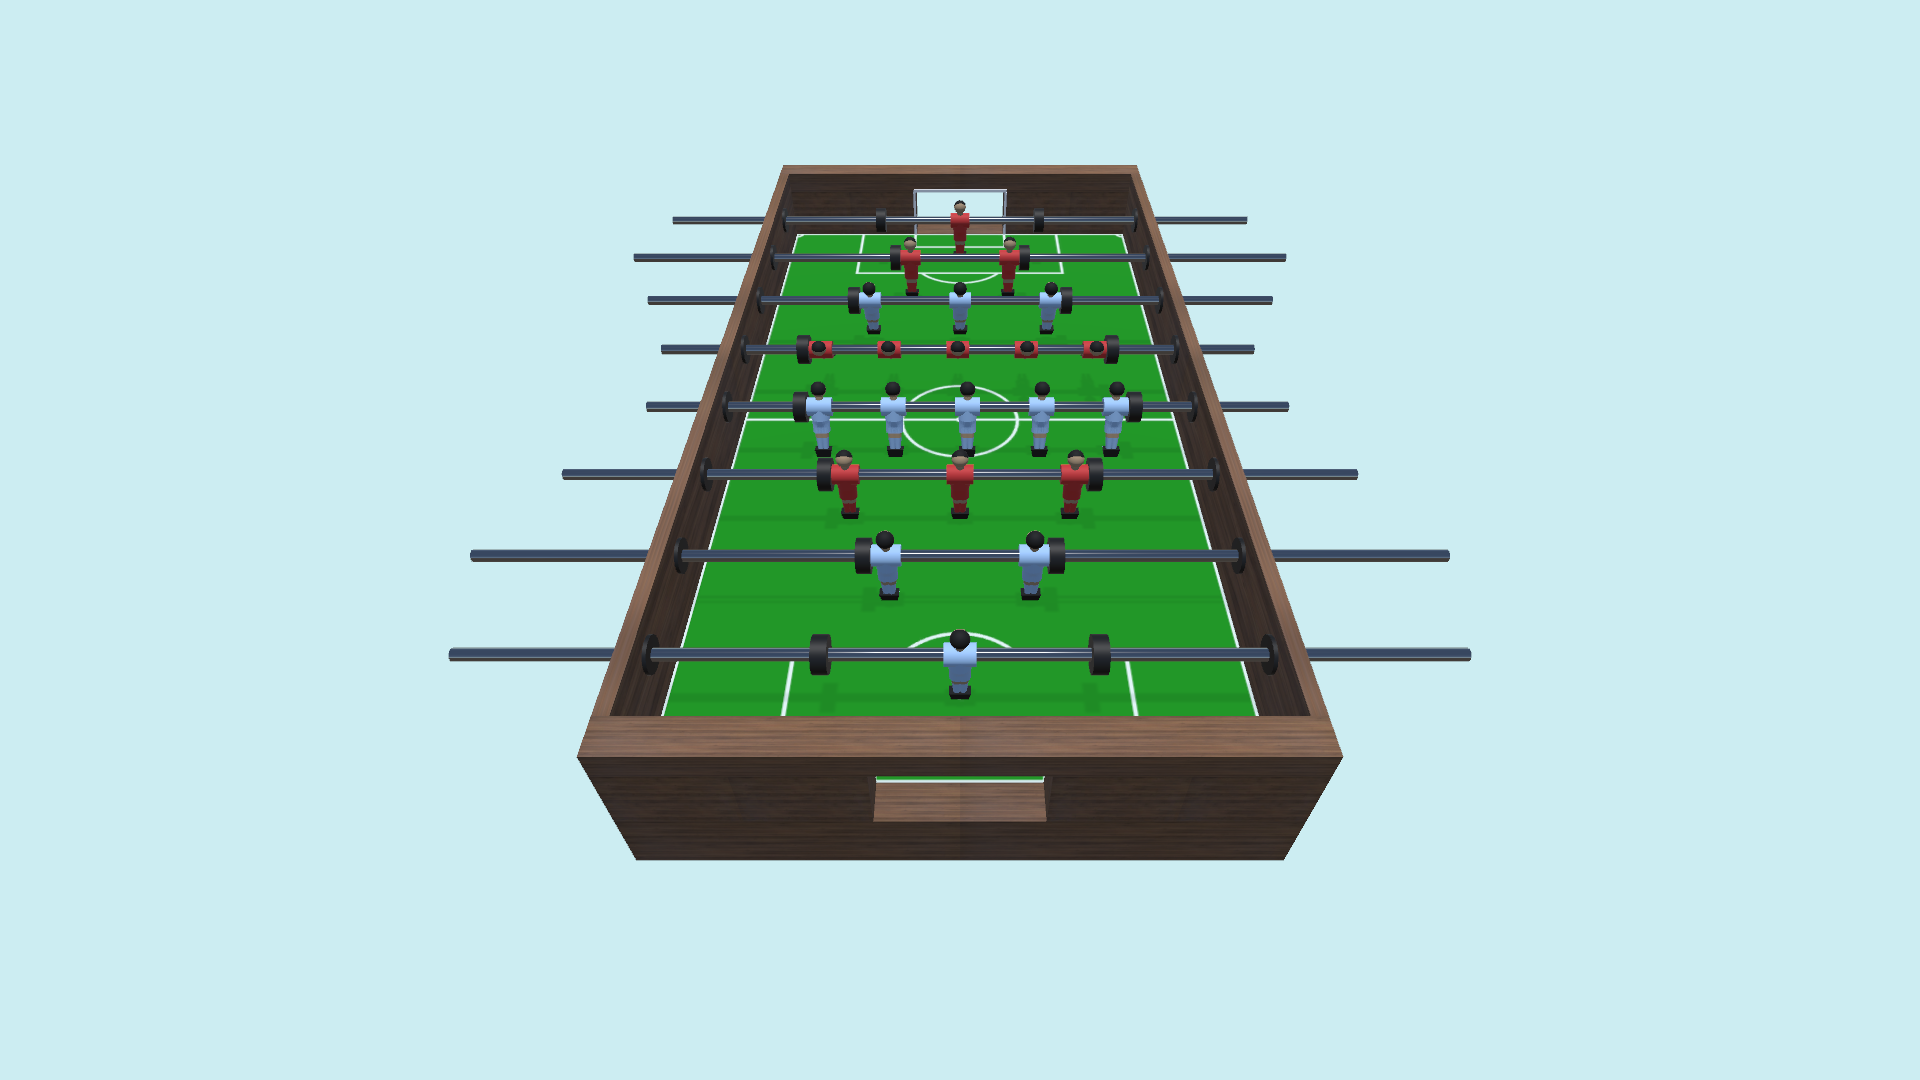
\includegraphics[width=0.47\textwidth]{image/app/env_football.png}\hfill
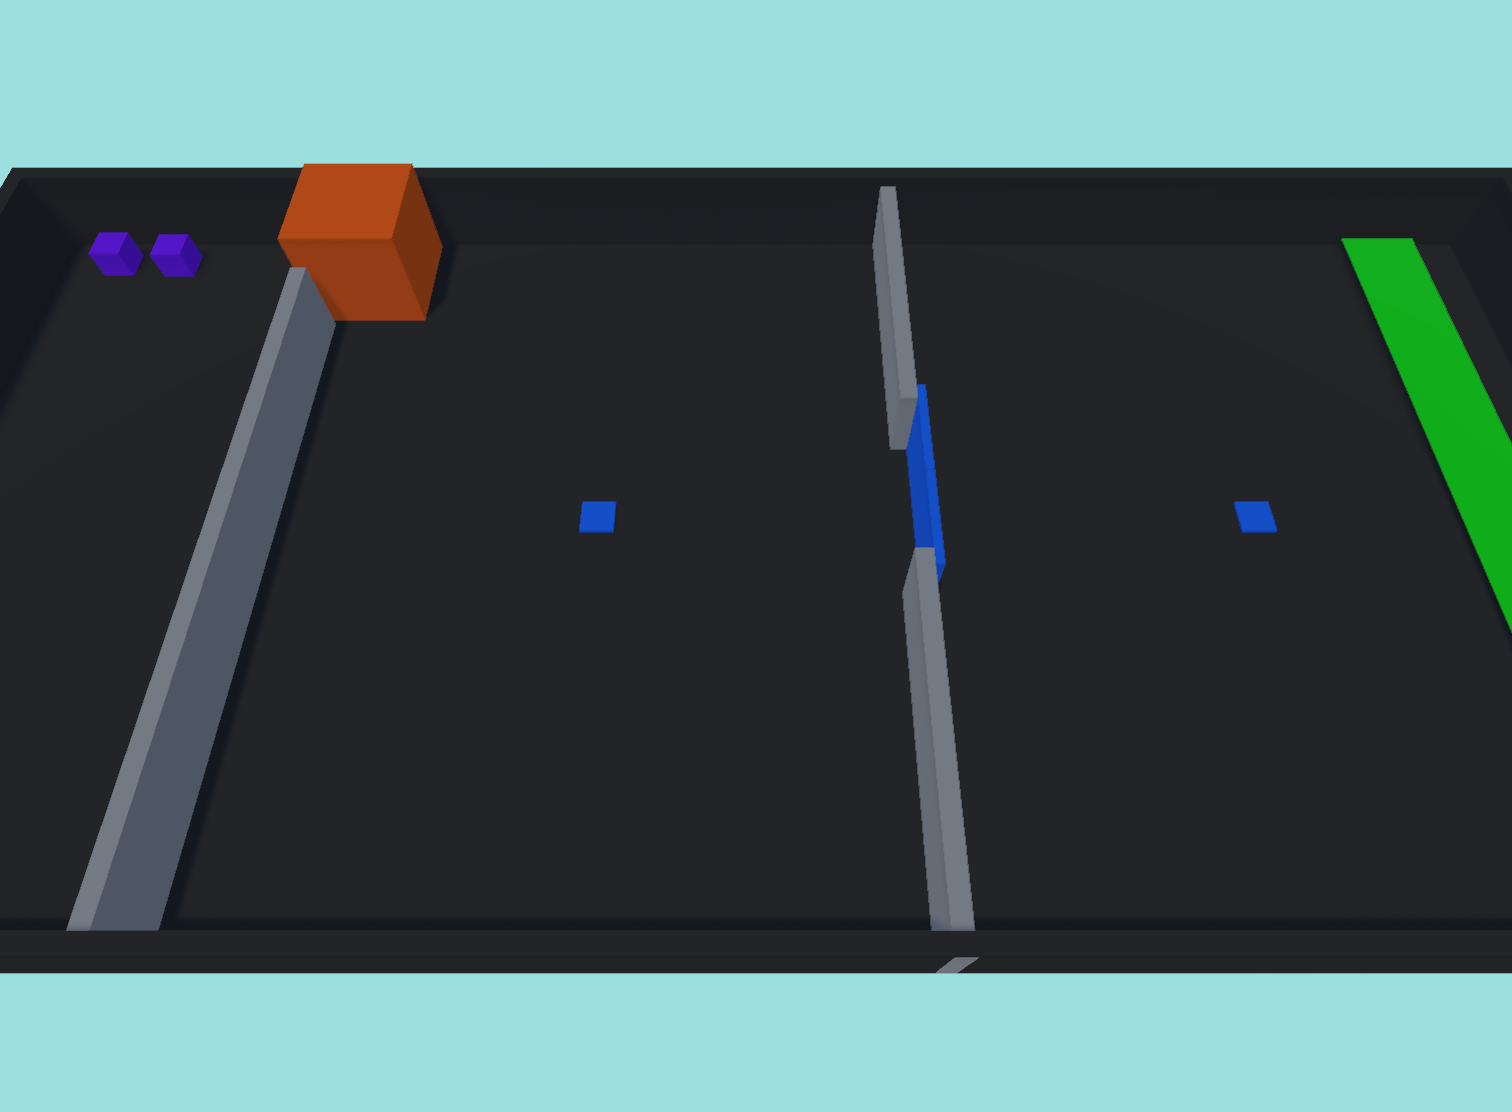
\includegraphics[width=0.47\textwidth]{image/app/env_puzzle.png}

\vspace{0.4cm}
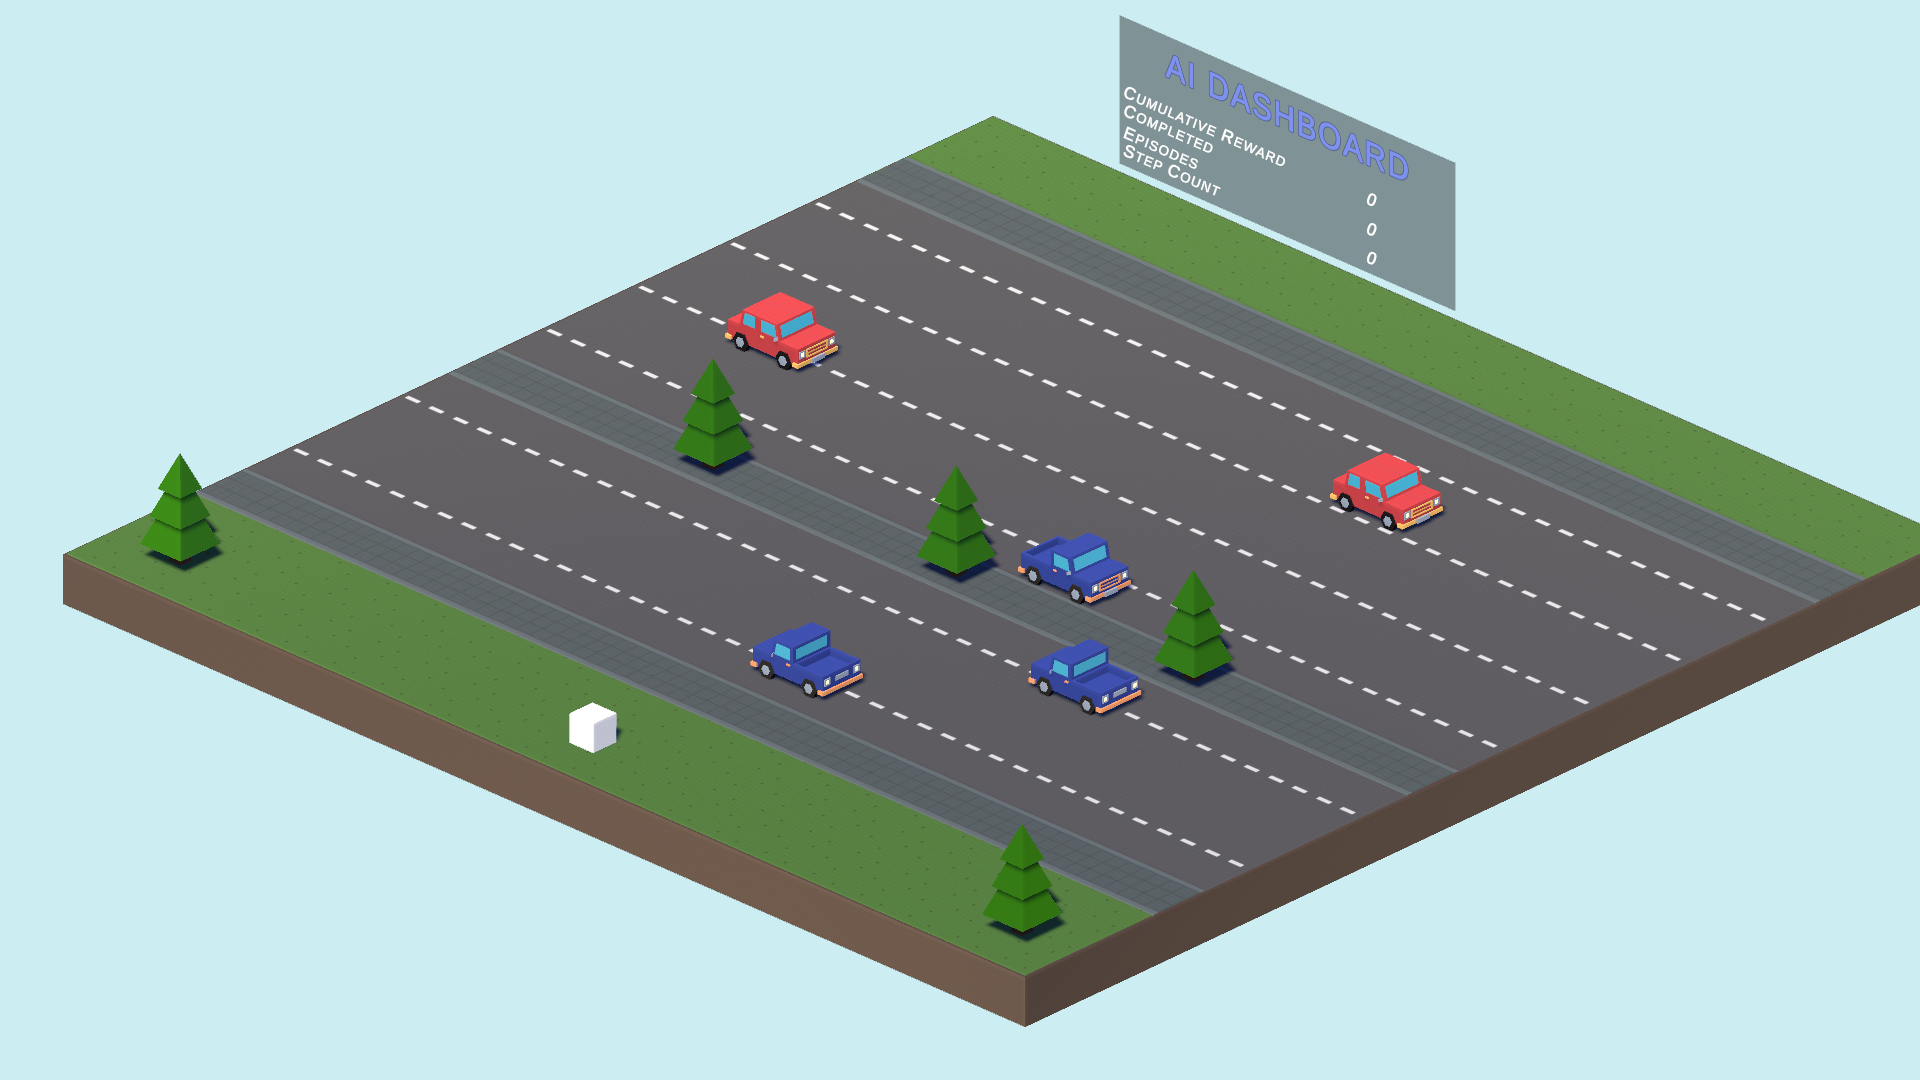
\includegraphics[width=0.47\textwidth]{image/app/env_crossroad.png}
\caption{Ba môi trường thực nghiệm. Trên trái: Football Table, hai đội Xanh - Đỏ mỗi
đội bốn thanh gạt. Trên phải: Capture The Flag, hai tác nhân phối hợp giữ cửa để cùng
tới đích. Dưới: Cross The Road, một tác nhân băng qua các làn xe đang chạy}
\label{fig:env_suite}
\end{figure}

\indent Tác nhân Football Table có tám hành động liên tục và sáu mươi quan
sát. Hàm phần thưởng gồm một phần thưởng lớn khi ghi bàn, một hình phạt khi bị thủng
lưới và một hình phạt thời gian nhỏ ở mỗi bước để thúc đẩy tác nhân dứt điểm sớm. Điều
kiện kết thúc được kích hoạt khi bóng vào một trong hai khung thành, hoặc khi lượt chơi
chạm mốc ba nghìn bước, tương ứng khoảng một phút mô phỏng.

\indent Tác nhân Capture The Flag có bảy hành động rời rạc và sáu mươi mốt
quan sát. Hàm phần thưởng gồm một phần thưởng nhóm khi cả hai tác nhân cùng tới đích,
một phần thưởng nhóm trao một lần cho mỗi tác nhân khi vượt được cổng đang khóa, một
phần thưởng cá nhân định hình theo thế năng khoảng cách tới đích, một phần thưởng nhỏ
khi đứng trên bàn đạp và một hình phạt thời gian nhóm ở mỗi bước. Điều kiện kết thúc
được kích hoạt khi cả hai tác nhân cùng chạm đích, hoặc khi khu vực huấn luyện chạy đủ
một trăm nghìn bước vật lý.

\indent Tác nhân Cross The Road có bốn hành động rời rạc và một trăm ba mươi
hai quan sát. Hàm phần thưởng gồm một phần thưởng khi chạm vạch đích và một hình phạt
nhỏ khi va chạm, kèm một tín hiệu tò mò cường độ thấp để khuyến khích khám phá. Điều
kiện kết thúc được kích hoạt ngay khi tác nhân chạm vạch đích hoặc va chạm với xe,
tường hay cây; lượt chơi không bị giới hạn số bước.

\indent Bảng~\ref{tab:env_speed} đối chiếu tốc độ huấn luyện thực đo của ba môi trường
trên cùng một máy. Chênh lệch giữa chúng rất lớn và bắt nguồn từ hai yếu tố: khối
lượng vật lý phải mô phỏng trong mỗi khu vực và số bước vật lý giữa hai lần ra quyết
định. Cross The Road chỉ mô phỏng một khối tác nhân trượt theo ô lưới cùng năm chiếc
xe chuyển động thẳng nên đạt tốc độ cao nhất. Football Table phải giải các khớp vật lý
của tám thanh gạt cùng va chạm liên tục của quả bóng nên chậm hơn gần mười lần. Capture
The Flag chậm nhất vì mỗi quyết định của tác nhân trải trên hai mươi bước vật lý và mỗi
lượt chơi kéo dài tới một trăm nghìn bước.

\begin{table}[H]
\centering
\caption{Tốc độ huấn luyện thực đo trên ba môi trường, mỗi môi trường lấy một lần chạy
đại diện; số bước là số bước huấn luyện của hành vi tương ứng}
\label{tab:env_speed}
\renewcommand{\arraystretch}{1.4}
\tablefont
\begin{tabular}{|p{2.9cm}|>{\centering\arraybackslash}p{2.2cm}
                |>{\centering\arraybackslash}p{1.85cm}
                |>{\centering\arraybackslash}p{2.05cm}
                |>{\centering\arraybackslash}p{1.45cm}
                |>{\centering\arraybackslash}p{1.85cm}|}
\hline
\textbf{Môi trường} & \textbf{Số bước huấn luyện} & \textbf{Thời gian} &
\textbf{Số bước mỗi giây} & \textbf{Quan sát} & \textbf{Hành động} \\
\hline
Football Table & 1.590.000 & 1 giờ 41 phút & 262 & 60 & 8 liên tục \\
\hline
Capture The Flag & 1.520.000 & 8 giờ 19 phút & 51 & 61 & 7 rời rạc \\
\hline
Cross The Road & 2.000.000 & 14 phút 32 giây & 2.294 & 132 & 4 rời rạc \\
\hline
\end{tabular}
\end{table}

% ═══════════════════════════════════════════════
\subsection{Môi trường Football Table}
\label{sub:env-football}

\subsubsection{Mô tả bài toán}
\indent Football Table mô phỏng một bàn bi lắc ba chiều với đầy đủ vật lý va chạm giữa
quả bóng và các cầu thủ gắn trên thanh gạt. Đây là bài toán đối kháng một đối một:
hai đội đối đầu trực tiếp, mỗi đội điều khiển bốn thanh gạt với mục tiêu đưa bóng vào
khung thành đối phương đồng thời bảo vệ khung thành của mình. Đặc trưng của bài toán
nằm ở tính đối kháng và ở động lực học liên tục của quả bóng: bóng lăn, nảy và đổi
hướng liên tục dưới tác động của va chạm, buộc tác nhân phải phản ứng nhanh và phải
học cả kỹ năng tấn công lẫn phòng thủ. Chính tính đối kháng khiến đây là trường hợp
điển hình để kiểm chứng cơ chế tự chơi, trong đó tác nhân tiến bộ bằng cách liên tục
thi đấu với những phiên bản ngày càng mạnh hơn của chính nó. Bố cục sân và hai bậc tự
do của mỗi thanh gạt được thể hiện trong Hình~\ref{fig:football_layout}.

\begin{figure}[H]
\centering
\begin{tikzpicture}[scale=0.7]
  % Field boundary
  \draw[thick] (0,0) rectangle (14,8);
  % Goals
  \fill[blue!20] (0,2.5) rectangle (0.5,5.5);
  \fill[red!20] (13.5,2.5) rectangle (14,5.5);
  \node[font=\small,rotate=90] at (0.25,4) {Khung thành};
  \node[font=\small,rotate=90] at (13.75,4) {Khung thành};
  % Rods with players - Blue team
  \foreach \x/\y in {2/4, 4/3, 6/5, 8/4} {
    \draw[thick,blue] (\x,0) -- (\x,8);
    \fill[blue] (\x,\y) circle (0.15);
    \fill[blue] (\x,\y+1.5) circle (0.15);
    \fill[blue] (\x,\y-1.5) circle (0.15);
  }
  % Rods with players - Red team
  \foreach \x/\y in {5/4, 7.5/4.5, 9.5/3.5, 12/4} {
    \draw[thick,red] (\x,0) -- (\x,8);
    \fill[red] (\x,\y) circle (0.15);
    \fill[red] (\x,\y+1.5) circle (0.15);
    \fill[red] (\x,\y-1.5) circle (0.15);
  }
  % Ball
  \fill[black] (7,4) circle (0.2);
  \node[below,font=\small] at (7,3.7) {Bóng};
  % Movement arrows
  \draw[<->,thick,blue] (2.5,0.5) -- (2.5,7.5) node[midway,right,font=\small] {Trượt};
  \draw[->,thick,red,rotate around={30:(8.5,4)}] (8.5,4) -- (9.5,4) node[right,font=\small] {Xoay};
\end{tikzpicture}
\caption{Sơ đồ bố cục sân và cơ chế điều khiển thanh gạt trong Football Table}
\label{fig:football_layout}
\end{figure}

\subsubsection{Không gian quan sát}
\label{sub:football-obs}
\indent Vector quan sát của mỗi đội gồm sáu mươi giá trị, chia thành ba nhóm bổ sung
cho nhau. Mười hai giá trị mô tả trạng thái quả bóng, gồm ba giá trị vận tốc đã nén về
khoảng $[-1,1]$ và chín giá trị mã hóa vị trí bóng. Ba mươi hai giá trị tiếp theo mô tả
trạng thái đội nhà: với mỗi thanh gạt, tác nhân quan sát vận tốc trượt, vận tốc xoay,
vị trí trượt và góc xoay hiện tại, tức đủ để biết chính xác tư thế của toàn bộ hàng cầu
thủ của mình. Mười sáu giá trị còn lại mô tả trạng thái đội đối phương với bốn đại lượng
tương tự cho mỗi thanh gạt, cho phép tác nhân dự đoán ý đồ và phản ứng của đối thủ.

\indent Hai chi tiết trong cách mã hóa quan sát đáng được nhấn mạnh. Kỹ thuật tách chữ
số thập phân thay việc đưa vào mạng một giá trị duy nhất cho vị trí bóng hay góc xoay
thanh gạt bằng cách tách giá trị đó thành nhiều thành phần ứng với các hàng thập phân
liên tiếp. Nhờ vậy, một thay đổi rất nhỏ ở hàng thập phân sâu vẫn tạo ra biến thiên rõ
rệt ở một thành phần đầu vào, giúp mạng nhạy hơn với các sai lệch tinh vi về vị trí, vốn
quyết định thành bại của một cú chạm bóng. Phép đối xứng hóa
quan sát thì đưa mọi vị trí và vận tốc về hệ tọa độ địa phương của sân rồi
nhân với một hệ số dấu tùy theo phía của đội. Sau phép biến đổi này, cả hai phía đều
thấy khung thành đối phương ở cùng một hướng quy ước, nhờ đó một chính sách duy nhất
vận hành được cho cả hai phía và cơ chế tự chơi trở nên nhất quán vì hai đội thực sự
dùng chung một mạng nơ-ron.

\indent Do các đại lượng vật lý trong môi trường này có thang đo chênh nhau nhiều bậc,
chế độ chuẩn hóa quan sát được bật trong cấu hình huấn luyện, theo đúng nguyên tắc ở
Mục~\ref{sub:obs-space}.

\subsubsection{Không gian hành động và cơ chế điều khiển}
\indent Mỗi đội được điều khiển bởi một tác nhân duy nhất, quản lý đồng thời cả bốn
thanh gạt. Tại mỗi bước quyết định, tác nhân xuất ra tám giá trị thực trong khoảng
$[-1,1]$; với mỗi thanh gạt có một giá trị điều khiển chuyển động trượt ngang để đưa
cầu thủ đến đúng vị trí và một giá trị điều khiển chuyển động xoay để thực hiện cú đá:
\begin{equation}
a = (f^{\text{trượt}}_1, f^{\text{xoay}}_1, \dots, f^{\text{trượt}}_4, f^{\text{xoay}}_4)
\in [-1, 1]^8 .
\end{equation}

\indent Việc gộp cả đội vào một tác nhân duy nhất, thay vì mỗi thanh gạt một tác nhân,
có hai lợi ích. Cách tổ chức này biến bài toán phối hợp giữa bốn thanh gạt thành một
bài toán điều khiển tập trung mà một chính sách duy nhất học được, tránh sự phức tạp
của việc đồng bộ nhiều tác nhân độc lập. Nó cũng phù hợp trực tiếp với cơ chế tự chơi,
vì khi đó mỗi phía của bàn chỉ cần đúng một chính sách để thi đấu.

\indent Về mặt vật lý, mỗi giá trị hành động không dịch chuyển thanh gạt tức thời mà
được diễn giải thành một mức thay đổi vận tốc trượt hoặc vận tốc xoay đặt lên thân vật
lý của thanh gạt tương ứng, với hệ số lần lượt là một và hai mươi lăm; hệ thống vật lý
của Unity mới quyết định chuyển động cuối cùng cùng va chạm giữa thanh gạt và quả bóng.
Tác nhân ra quyết định sau mỗi hai bước vật lý, tức hai mươi lăm quyết định mỗi giây mô
phỏng, và hành động được giữ nguyên ở bước vật lý xen giữa. Chính tính liên tục này
khiến Football Table trở thành phép thử tiêu biểu cho các thuật toán điều khiển liên
tục, khác hẳn hai môi trường rời rạc còn lại.

\subsubsection{Hàm phần thưởng}
\indent Hàm phần thưởng của môi trường được tổng hợp trong
Bảng~\ref{tab:reward_football}. Chiếu theo khuôn dạng~\eqref{eq:reward-decomp}, môi
trường này chỉ dùng hai lớp: một thành phần mục tiêu thưa tại trạng thái kết thúc,
gồm cộng năm điểm khi ghi bàn và trừ một điểm khi bị thủng lưới, cùng một thành phần
theo bước là hình phạt thời gian bằng $1/3000$ điểm ở mỗi bước. Thành phần định hình
theo thế năng không được sử dụng, vì lý do trình bày ở cuối mục này.

\indent Việc đặt phần thưởng ghi bàn lớn gấp năm lần hình phạt thủng lưới không phải
một lựa chọn tùy ý mà xuất phát từ đặc thù của bài toán đối kháng: với hàm phần thưởng
đối xứng, chính sách an toàn nhất là giữ bóng ở phần sân nhà và không bao giờ dâng lên,
bởi mọi pha tấn công đều mở ra nguy cơ phản công. Có thể lượng hóa nhận định này. Xét
một tình huống mà tác nhân có thể chọn giữa cầm cự, tức giữ bóng đến hết lượt
chơi, và dứt điểm, tức tổ chức một pha tấn công thành công với xác suất $p$ và
bị phản công thủng lưới với xác suất $1 - p$. Gọi $R_{+}$ là phần thưởng ghi bàn,
$R_{-}$ là hình phạt thủng lưới và bỏ qua hình phạt thời gian trong nhánh dứt điểm vì
lượt chơi kết thúc sớm, giá trị kỳ vọng của hai lựa chọn là
\begin{equation}
V_{\text{cầm cự}} = -\,T \cdot \frac{1}{3000} = -1 ,
\qquad
V_{\text{dứt điểm}} = p\,R_{+} - (1-p)\,R_{-} ,
\label{eq:football-tradeoff}
\end{equation}
với $T = 3000$ là số bước tối đa của một lượt chơi. Lối chơi tấn công chỉ được ưa
chuộng khi $V_{\text{dứt điểm}} > V_{\text{cầm cự}}$, tức khi
\begin{equation}
p > \frac{R_{-} - 1}{R_{+} + R_{-}} .
\label{eq:football-threshold}
\end{equation}
Với cấu hình đối xứng $R_{+} = R_{-} = 5$, ngưỡng này bằng $0{,}4$: tác nhân chỉ chịu
tấn công khi tự tin thắng ít nhất bốn mươi phần trăm số pha bóng, một điều gần như
không bao giờ đúng ở giai đoạn đầu huấn luyện, nên chính sách hội tụ về phòng ngự tuyệt
đối. Với cấu hình được chọn $R_{+} = 5$ và $R_{-} = 1$, ngưỡng tụt xuống đúng bằng
không: mọi cơ hội ghi bàn dù nhỏ đến đâu cũng đáng để thử. Đây chính là lý do của tỉ lệ
năm trên một, và nó cũng cho thấy hình phạt thời gian không phải một chi tiết phụ mà là
thành phần quyết định dấu của vế phải trong~\eqref{eq:football-threshold}.

\indent Giá trị $1/3000$ của hình phạt thời gian được chọn theo nguyên tắc giữ trật tự
độ lớn ở Mục~\ref{sub:reward-principle}: nhân với $T = 3000$ bước, tổng phạt tích lũy
trọn một lượt chơi bằng đúng một điểm, tức bằng đúng hình phạt thủng lưới. Cách chuẩn
hóa này tạo ra một hệ quả có chủ đích: một lượt chơi hòa không bàn thắng bị đánh giá
ngang bằng với việc để thủng lưới một bàn, nên tác nhân không thể coi thế trận bế tắc là
một kết quả chấp nhận được. Đồng thời tổng phạt vẫn nhỏ hơn nhiều phần thưởng ghi bàn,
nên nó không bao giờ lấn át được mục tiêu chính.

\begin{table}[H]
\centering
\caption{Hàm phần thưởng của môi trường Football Table}
\label{tab:reward_football}
\renewcommand{\arraystretch}{1.4}
\tablefont
\begin{tabular}{|p{6cm}|>{\centering\arraybackslash}p{3cm}|p{4cm}|}
\hline
\textbf{Sự kiện} & \textbf{Giá trị} & \textbf{Loại} \\
\hline
Ghi bàn vào khung thành đối phương & $+5{,}0$ & Thưởng mục tiêu \\
\hline
Bị thủng lưới & $-1{,}0$ & Phạt mục tiêu \\
\hline
Mỗi bước trôi qua & $-1/3000$ & Phạt thời gian \\
\hline
\end{tabular}
\end{table}

\indent Mã nguồn của tác nhân còn cài đặt sẵn hai thành phần định hướng tùy chọn: một
phần thưởng tỉ lệ với thành phần vận tốc của bóng chiếu lên hướng nối tới khung thành
đối phương, chỉ kích hoạt khi tác nhân đang kiểm soát bóng, và một hình phạt khi thanh
gạt xoay quá mạnh. Trong toàn bộ các lần huấn luyện được báo cáo ở
Chương~\ref{ch:results}, hai hệ số này đều được đặt bằng không, tức hai thành phần
không tham gia vào tín hiệu học. Quyết định này có ba căn cứ.

\indent Phần thưởng theo vận tốc bóng không có dạng thế năng. Nó phụ thuộc vào
vận tốc, tức một đại lượng của phép chuyển chứ không phải một hàm của riêng trạng thái,
nên không thể viết thành $\gamma\,\Phi(s') - \Phi(s)$ và do đó nằm ngoài phạm vi bảo đảm
bất biến của Định nghĩa~\ref{dn:pbrs}. Hệ quả trực tiếp là đẳng thức~\eqref{eq:pbrs-cycle}
không còn đúng: tác nhân hoàn toàn có thể đẩy bóng tới lui theo hướng khung thành đối
phương để tích lũy phần thưởng vô hạn mà không bao giờ dứt điểm, đúng theo cơ chế đã
quan sát được trong thí nghiệm xe đạp của Randløv và Alstrøm \cite{randlov1998learning}.

\indent Hình phạt xoay mạnh vi phạm nguyên tắc bám theo lời giải mẫu. Một cú sút mạnh
bắt buộc phải đi kèm vận tốc xoay lớn của thanh gạt, nên khoản phạt này giáng đúng vào
hành động nằm trên quỹ đạo hoàn thành nhiệm vụ; giữ nó ở mức khác không sẽ đẩy tác nhân
về lối chơi rê bóng chậm chạp thay vì dứt điểm.

\indent Cuối cùng, cơ chế tự chơi đã tự cung cấp một chương trình học có độ khó tăng dần
mà không cần bất kỳ tín hiệu định hướng thủ công nào: đối thủ luôn mạnh tương đương với
tác nhân ở thời điểm hiện tại, nên tỉ lệ thắng thua giữ ở mức cân bằng và tín hiệu thưa
vẫn xuất hiện đủ thường xuyên để việc học tiến triển. Đây chính là lập luận đã được
kiểm chứng ở quy mô lớn hơn nhiều trong AlphaGo Zero \cite{silver2017mastering}, nơi một
chính sách mạnh hơn con người được học chỉ từ tín hiệu thắng thua ở cuối ván mà không có
bất kỳ phần thưởng trung gian nào. Giữ nguyên hai thành phần trong mã nguồn cho phép bật
lại khi cần khảo sát ảnh hưởng của phần thưởng định hướng.

\subsubsection{Điều kiện kết thúc lượt chơi}
\indent Một lượt chơi kết thúc khi có bàn thắng, tức bóng đi vào một trong hai khung
thành; khi đó cả hai tác nhân nhận phần thưởng tương ứng rồi lượt chơi được đặt lại,
bóng và các thanh gạt trở về vị trí ban đầu. Lượt chơi cũng kết thúc khi chạm mốc ba
nghìn bước, tương ứng khoảng một phút mô phỏng; giới hạn này ngăn những thế trận bế tắc
kéo dài vô hạn và bảo đảm dữ liệu huấn luyện luôn được làm mới.

\subsubsection{Cấu hình huấn luyện}
\indent Do bản chất đối kháng và không gian hành động liên tục, môi trường này được
huấn luyện chính bằng PPO kết hợp cơ chế tự chơi. Mạng chính sách gồm hai lớp ẩn với
hai trăm năm mươi sáu đơn vị mỗi lớp và bật chuẩn hóa quan sát. Cơ chế tự chơi được cấu
hình để lưu lại một phiên bản đối thủ sau mỗi năm mươi nghìn bước, đổi phía sau mỗi một
trăm nghìn bước, giữ một cửa sổ mười đối thủ gần nhất với xác suất đấu với phiên bản
mới nhất là một nửa, và theo dõi tiến bộ qua chỉ số xếp hạng khởi tạo ở mức một nghìn
hai trăm. Số bước huấn luyện tối đa được đặt ở mười triệu bước. Hai thuật toán còn lại
được đưa vào so sánh là SAC và MA-POCA, huấn luyện dưới cùng điều kiện để bảo đảm mặt
bằng so sánh công bằng. Cấu hình siêu tham số đầy đủ được liệt kê trong các Phụ lục A,
B và C.

% ═══════════════════════════════════════════════
\subsection{Môi trường Capture The Flag}
\label{sub:env-coop}

\subsubsection{Mô tả bài toán}
\indent Capture The Flag là một câu đố không gian mang tính hợp tác, trong đó hai tác
nhân phải phối hợp chặt chẽ để cùng về đích. Điểm mấu chốt là nhiệm vụ được thiết kế
sao cho không một tác nhân nào có thể tự mình hoàn thành: để đi từ khu vực xuất
phát tới đích, cả hai bắt buộc phải thực hiện một màn bàn giao, trong đó lần lượt mỗi
tác nhân giữ cửa mở cho tác nhân kia đi qua. Sự phụ thuộc lẫn nhau này biến bài toán
thành trường hợp điển hình để làm nổi bật thách thức gán công lao trong học tăng cường
hợp tác, tức việc xác định đóng góp thực sự của từng tác nhân vào thành quả chung của
cả nhóm; đây cũng chính là dạng bài toán mà MA-POCA được thiết kế để giải quyết.

\indent Bố cục không gian, thể hiện trong Hình~\ref{fig:puzzle_layout}, là một hành
lang dài trải theo một trục, được chia thành ba khoang bởi hai bức tường ngăn có khe hở
lệch nhau. Khoang đầu tiên là phòng xuất phát, nơi hai tác nhân và một khối vật cản
được đặt ban đầu; lối ra khỏi khoang này là một khe hở nằm lệch về một bên của bức
tường ngăn thứ nhất. Khoang ở giữa chứa bàn đạp áp lực thứ nhất. Ngăn cách khoang giữa
với khoang cuối là một cổng cửa nằm ở khe hở chính giữa của bức tường
ngăn thứ hai; cổng gồm hai cánh cửa có thể hạ xuống để mở và nâng lên để chặn. Khoang
cuối chứa bàn đạp áp lực thứ hai và, ở tận cùng, là vạch đích trải suốt chiều rộng
hành lang. Điểm thiết kế cốt lõi là cả hai bàn đạp đều điều khiển chung một cổng
cửa, và chúng nằm ở hai phía đối diện của cổng: bàn đạp thứ nhất ở phía trong, cùng
khoang với điểm xuất phát; bàn đạp thứ hai ở phía ngoài, đã qua cổng. Chính sự bố trí
đối xứng này tạo nên cấu trúc bàn giao mà lời giải bắt buộc phải tuân theo.

\begin{figure}[H]
\centering
\begin{tikzpicture}[scale=0.8]
  % Vòng ngoài hành lang
  \draw[thick] (0,0) rectangle (12,4);

  % Tường ngăn 1
  \draw[thick] (4,0) -- (4,2.5);
  \draw[thick] (4,3.5) -- (4,4);

  % Tường ngăn 2 (Cổng)
  \draw[thick] (8,0) -- (8,1.5);
  \draw[thick] (8,2.5) -- (8,4);
  \draw[ultra thick,red] (8,1.5) -- (8,2.5) node[midway,right,font=\footnotesize,black] {Cổng};

  % Bàn đạp 1 và 2
  \fill[orange] (6,3) circle (0.25) node[above=2pt,font=\footnotesize,black] {Bàn đạp 1};
  \fill[orange] (9.5,1) circle (0.25) node[below=2pt,font=\footnotesize,black] {Bàn đạp 2};

  % Tác nhân
  \fill[blue] (1,2) ++(0:0.3) -- ++(120:0.6) -- ++(240:0.6) -- cycle;
  \fill[blue] (2,2) ++(0:0.3) -- ++(120:0.6) -- ++(240:0.6) -- cycle;

  % Đích
  \fill[green!50!black] (11.5,0) rectangle (12,4);
  \node[font=\footnotesize,rotate=90,white] at (11.75,2) {Đích};

  % Mũi tên bàn giao
  \draw[->,dashed,thick,blue] (2.5,2.2) to[out=30,in=180] (5.7,3);
  \draw[->,dashed,thick,blue] (1.5,1.8) to[out=-30,in=180] (7.8,2) to[out=0,in=150] (9.2,1);
\end{tikzpicture}
\caption{Sơ đồ bố cục không gian và trình tự bàn giao trong Capture The Flag}
\label{fig:puzzle_layout}
\end{figure}

\subsubsection{Không gian quan sát}
\label{sub:coop-obs}
\indent Quan sát của mỗi tác nhân gồm sáu mươi mốt giá trị đến từ ba nguồn bổ sung cho
nhau. Bốn giá trị đầu là các cờ nhị phân mang tính logic: bàn đạp thứ nhất đã được nhấn
hay chưa, bàn đạp thứ hai đã được nhấn hay chưa, bản thân tác nhân đã vượt qua cổng hay
chưa, và đồng đội đã vượt qua cổng hay chưa. Hai cờ đầu cho tác nhân biết cửa hiện có
đang được giữ mở hay không mà không cần nhìn thấy cổng; hai cờ sau chính là mấu chốt để
một tác nhân biết khi nào nên rời bàn đạp, bởi chỉ khi đồng đội đã sang bên kia thì
việc nhả bàn đạp mới hợp lý. Nếu thiếu cờ trạng thái của đồng đội, chính sách phi tập
trung không có căn cứ trực tiếp để định thời điểm bàn giao và bài toán trở nên khó học
hơn nhiều. Kèm theo đó là một cờ nhị phân riêng ghi nhận tác nhân đã chạm đích hay
chưa.

\indent Năm mươi sáu giá trị còn lại đến từ cảm biến tia mô tả ở
Mục~\ref{sub:obs-space}. Cấu hình cụ thể gồm bảy tia trải trong góc quạt bảy mươi độ
phía trước, tầm xa hai mươi đơn vị, nhận diện sáu nhãn vật thể là đồng đội, tường, khối
vật cản, bàn đạp, cửa và đích. Mỗi tia sinh ra sáu giá trị mã hóa một-nóng cho nhãn,
một giá trị báo tia có chạm vật thể nào không và một giá trị khoảng cách chuẩn hóa, tức
tám giá trị cho mỗi tia. Nhờ cảm biến này, tác nhân nhận biết được cấu trúc không gian
xung quanh cùng vị trí tương đối của đồng đội trong tầm nhìn mà không cần được cung cấp
tọa độ tuyệt đối. Sự kết hợp giữa các cờ logic tường minh và quan sát không gian cho
phép tác nhân vừa suy luận về trạng thái phối hợp của cả nhóm, vừa điều hướng chính xác
trong hành lang hẹp.

\subsubsection{Không gian hành động và cơ chế điều khiển}
\indent Mỗi tác nhân điều khiển một khối hộp có thân vật lý, di chuyển trong không gian
ba chiều bằng bảy hành động rời rạc: đứng yên, tiến, lùi, xoay trái, xoay phải, đi
ngang sang trái và đi ngang sang phải. Tập hành động này đủ phong phú để tác nhân vừa
di chuyển linh hoạt vừa định hướng chính xác khi cần đứng vào đúng vị trí bàn đạp. Đúng
như đã nêu ở Mục~\ref{sub:action-space}, mỗi lệnh di chuyển không dịch chuyển tác nhân
tức thời mà cộng thêm một lượng vận tốc bằng $1{,}4$ đơn vị trên giây vào thân vật lý
theo hướng tương ứng ở mỗi bước vật lý, trong khi hệ số cản tuyến tính được đặt ở mức
bốn để liên tục hãm vận tốc lại. Hai lệnh xoay làm tác nhân quay quanh trục đứng với
tốc độ hai trăm độ mỗi giây. Tác nhân ra quyết định sau mỗi hai mươi bước vật lý, tức
hai phẩy năm quyết định mỗi giây mô phỏng, và hành động được giữ nguyên ở các bước vật
lý xen giữa.

\indent Sự cân bằng giữa lượng vận tốc cộng thêm và hệ số cản làm cho tác nhân có một
vận tốc tối đa hữu hạn thay vì tăng tốc vô hạn. Ở trạng thái dừng, vận tốc tối đa đạt
được là
\begin{equation}
v_{\max} = \frac{\Delta v}{c \cdot \Delta t}
         = \frac{1{,}4}{4 \times 0{,}02} = 17{,}5 \text{ đơn vị/giây},
\label{eq:vmax}
\end{equation}
với $\Delta v$ là lượng vận tốc cộng thêm mỗi bước, $c$ là hệ số cản và $\Delta t$ là
độ dài một bước vật lý. Ngoài ý nghĩa vật lý thuần túy, giá trị này còn là yếu tố then
chốt bảo đảm tính đúng đắn của cơ chế bàn giao, như sẽ phân tích ngay dưới đây.

\subsubsection{Cơ chế cửa và pha bàn giao}
\label{sub:coop-handoff}
\indent Cổng cửa chỉ mở khi có tác nhân đang đứng trên một trong hai bàn đạp. Tuy nhiên,
nếu cửa đóng lại ngay lập tức vào đúng khoảnh khắc tác nhân rời bàn đạp thì màn bàn
giao gần như không thể khám phá được bằng thử - sai, vì nó đòi hỏi một sự đồng bộ thời
gian hoàn hảo. Để hành vi hợp tác trở nên khả học, đề tài đưa vào một khoảng ân hạn:
sau khi tác nhân rời khỏi bàn đạp, cửa vẫn giữ mở thêm một giây mô phỏng rồi mới đóng.
Khoảng ân hạn này tạo ra một cửa sổ thời gian đủ để đồng đội kịp lên giữ bàn đạp còn
lại, qua đó làm mượt quá trình học mà không làm thay đổi bản chất bài toán.

\indent Một câu hỏi thiết kế quan trọng là liệu khoảng ân hạn có vô tình cho phép một
tác nhân tự mình vượt cổng hay không, tức bước lên bàn đạp thứ nhất rồi chạy
thật nhanh qua cổng trước khi cửa kịp đóng, khiến sự hợp tác trở nên không cần thiết.
Có thể loại trừ khả năng này bằng một lập luận định lượng. Khoảng cách từ bàn đạp thứ
nhất tới cổng là mười chín đơn vị, trong khi khoảng ân hạn chỉ dài một giây. Ngay cả
khi giả định tác nhân đã chạy sẵn ở vận tốc tối đa $17{,}5$ đơn vị trên giây theo công
thức~\eqref{eq:vmax}, quãng đường nó đi được trong một giây vẫn nhỏ hơn mười chín đơn
vị. Trên thực tế tác nhân xuất phát từ trạng thái đứng yên trên bàn đạp và phải mất
thời gian tăng tốc, nên quãng đường thực tế chỉ khoảng mười ba phẩy hai đơn vị, tức
chưa tới bảy mươi phần trăm khoảng cách cần vượt. Do đó không tồn tại quỹ đạo nào giúp
một tác nhân đơn độc vượt cổng trong khoảng ân hạn. Kết luận này bảo đảm rằng mọi lần
vượt cổng thành công đều là bằng chứng của sự hợp tác thực sự, chứ không phải của một
lối tắt cá nhân; nó cũng là cơ sở để diễn giải đúng các chỉ số phần thưởng ở
Chương~\ref{ch:results}.

\subsubsection{Hàm phần thưởng}
\indent Đây là môi trường có hàm phần thưởng phức tạp nhất của đề tài, và cũng là môi
trường duy nhất phải trải qua một vòng thiết kế lại sau khi phiên bản đầu tiên thất bại.
Mục này trình bày thiết kế cuối cùng cùng lý do của từng thành phần;
Mục~\ref{sub:coop-reward-process} thuật lại quá trình đi tới thiết kế đó.

\indent Điểm xuất phát của toàn bộ thiết kế là lời giải mẫu, theo đúng nguyên
tắc bám theo lời giải mẫu ở Mục~\ref{sub:reward-principle}. Với bố cục đã mô tả, một
lượt chơi thành công bắt buộc phải đi qua chuỗi trạng thái sau: hai tác nhân rời phòng
xuất phát; một tác nhân bước lên bàn đạp phía trong và đứng yên giữ cửa; tác nhân còn
lại vượt cổng; tác nhân vừa vượt cổng bước lên bàn đạp phía ngoài để giữ cửa ngược lại;
tác nhân đang đứng ở bàn đạp phía trong rời chỗ và vượt cổng; cuối cùng cả hai cùng tiến
tới vạch đích.
Mọi thành phần phần thưởng đều được kiểm tra đối chiếu với chuỗi này, và yêu cầu bắt
buộc là không thành phần nào được phạt một trạng thái nằm trên chuỗi. Yêu cầu tưởng
chừng hiển nhiên này chính là điều mà phiên bản phần thưởng đầu tiên vi phạm.

\indent \textbf{Phần thưởng mục tiêu.} Khoản lớn nhất, bằng một điểm, chỉ được trao khi
cả hai tác nhân cùng đến được đích, và được trao cho nhóm chứ không cho cá nhân.
Việc chọn phạm vi nhóm là một quyết định có hệ quả sâu xa: nó khiến hàm giá trị mà mạng
phê bình phải học trở thành giá trị của cả đội, nhờ đó một tác nhân đứng yên giữ bàn đạp
vẫn được ghi nhận công lao khi đồng đội về đích. Nếu trao phần thưởng theo cá nhân, tác
nhân giữ cửa sẽ không nhận được gì cho hành vi hy sinh của mình và chính sách sẽ nhanh
chóng học cách bỏ mặc đồng đội. Chính cấu hình phần thưởng nhóm này là điều kiện để các
thuật toán gán công lao đa tác nhân như MA-POCA \cite{cohen2022mapoca} phát huy tác
dụng, vì phê bình tập trung của chúng được thiết kế để phân rã một phần thưởng chung
thành đóng góp của từng tác nhân \cite{foerster2018counterfactual}.

\indent \textbf{Phần thưởng định hình theo khoảng cách.} Thành phần dẫn đường được xây
dựng đúng theo khuôn khổ ở Định nghĩa~\ref{dn:pbrs}, với hàm thế năng lấy bằng đối số
của khoảng cách từ tác nhân tới đích, $\Phi(s) = -d(s)$. Phần thưởng cộng thêm ở mỗi
bước do đó có dạng
\begin{equation}
F(s_{t-1}, s_t) = \kappa\,\bigl[d(s_{t-1}) - d(s_t)\bigr], \qquad \kappa = 0{,}01 ,
\label{eq:ctf-pbrs}
\end{equation}
tức thưởng cho mỗi bước rút ngắn khoảng cách và phạt cho mỗi bước nới rộng nó. Cài đặt
dùng hiệu thế năng thuần túy thay vì dạng chiết khấu $\gamma\,\Phi(s') - \Phi(s)$; với
$\gamma = 0{,}99$ trong cấu hình huấn luyện, sai khác giữa hai dạng là $(1-\gamma)\Phi$,
nhỏ hơn hai bậc so với chính tín hiệu dẫn đường, nên tính bất biến chính sách vẫn được
bảo toàn ở mức xấp xỉ có thể chấp nhận \cite{devlin2012dynamic}. Ba hệ quả của lựa chọn
này đáng được nêu rõ. Tín hiệu dẫn đường phủ kín toàn bộ hành lang, kể cả những đoạn
không có cột mốc nào, nên tác nhân không bao giờ rơi vào vùng hoàn toàn không có gradient
học. Đẳng thức~\eqref{eq:pbrs-cycle} bảo đảm mọi hành vi đi tới đi lui đều cho lợi ích
ròng bằng không, nên thành phần này không thể bị lợi dụng. Và quan trọng nhất đối với
bài toán hợp tác, một tác nhân đứng yên giữ bàn đạp có $d(s_t) = d(s_{t-1})$ nên
không bị thành phần này phạt, tức hành vi hy sinh nằm trên lời giải mẫu được giữ trung
lập thay vì bị trừng phạt.

\indent Tổng phần thưởng định hình mà một tác nhân có thể thu về trong trọn một lượt
chơi được xác định hoàn toàn bởi tính chất khớp nối của tổng~\eqref{eq:pbrs-cycle}:
\begin{equation}
\sum_{t=1}^{T} F(s_{t-1}, s_t)
= \kappa\,\bigl[d(s_0) - d(s_T)\bigr] \le \kappa\, d(s_0) ,
\label{eq:ctf-shaping-bound}
\end{equation}
tức chỉ phụ thuộc vào khoảng cách ban đầu chứ không phụ thuộc vào độ dài lượt chơi hay
vào quỹ đạo mà tác nhân chọn. Hệ số $\kappa = 0{,}01$ được chọn theo đúng ràng buộc
này: để thành phần dẫn đường không lấn át phần thưởng mục tiêu, cần $\kappa\,d(s_0) < 1$,
tức $d(s_0) < 100$ đơn vị, điều mà chiều dài hành lang của bố cục hiện tại thỏa mãn với
biên độ an toàn rộng rãi.

\indent \textbf{Phần thưởng bàn giao.} Thành phần hợp tác then chốt được trao mỗi khi
một tác nhân vừa vượt qua cổng đang khóa: cả nhóm được cộng nửa điểm, và mỗi tác
nhân chỉ nhận khoản này một lần duy nhất trong mỗi lượt chơi. Ba chi tiết trong định
nghĩa trên đều có lý do. Điều kiện cổng đang khóa, kết hợp với kết luận định lượng ở
Mục~\ref{sub:coop-handoff} rằng không tồn tại quỹ đạo giúp một tác nhân đơn độc vượt
cổng, khiến sự kiện kích hoạt phần thưởng tương đương logic với sự kiện hợp tác
thành công; nhờ vậy tín hiệu không phải một đại lượng thay thế gần đúng cho hành vi mong
muốn mà là chỉ báo chính xác của nó, tránh được đúng cái bẫy mà Amodei và cộng sự
\cite{amodei2016concrete} cảnh báo. Phạm vi nhóm bảo đảm tác nhân đang giữ bàn đạp cũng
được ghi nhận công lao cho cú vượt cổng của đồng đội. Còn đặc tính một lần khiến khoản
thưởng không thể bị khai thác bằng cách lặp lại động tác ra vào cổng, khác hẳn một khoản
cộng dồn theo từng bước; đây chính là bài học rút ra từ phiên bản thiết kế đầu tiên.

\indent \textbf{Các khoản theo bước.} Một khoản thưởng nhỏ được trao cho tác nhân đang
đứng trên bàn đạp, và một khoản tương tự cho việc đẩy khối vật cản. Hai khoản này cố ý
đi ngược nguyên tắc ưu tiên sự kiện một lần, vì lý do khám phá: giữ bàn đạp là một hành
vi phải được duy trì theo thời gian nên không thể diễn đạt bằng một sự kiện tức
thời, và nếu không có tín hiệu nào cho nó thì xác suất để tác nhân tình cờ đứng yên đủ
lâu trên bàn đạp là quá nhỏ. Rủi ro nấn ná được khống chế bằng cách chuẩn hóa theo độ
dài lượt chơi: khoản thưởng bằng $0{,}5/N$ mỗi bước, nên ngay cả khi tác nhân đứng lì
trên bàn đạp suốt lượt chơi, tổng thu về cũng chỉ đúng $0{,}5$ điểm, thấp hơn hẳn mức
$1{,}5$ điểm mà nó nhận được nếu tham gia trọn vẹn một lời giải bàn giao. Cuối cùng, một
khoản phạt thời gian nhóm bằng $0{,}1/N$ mỗi bước thúc đẩy nhóm hoàn thành nhanh hơn;
giá trị này được giữ rất nhỏ để tổng phạt trọn lượt chơi chỉ là $0{,}1$ điểm, đủ để phá
thế hòa giữa hai chính sách cùng hoàn thành nhiệm vụ nhưng không đủ để chi phối tín hiệu
học, một sai lầm mà phiên bản đầu tiên đã mắc phải.

\begin{table}[H]
\centering
\caption{Hàm phần thưởng của môi trường Capture The Flag}
\label{tab:reward_capture}
\renewcommand{\arraystretch}{1.4}
\tablefont
\begin{tabular}{|p{7cm}|>{\centering\arraybackslash}p{3.4cm}|>{\centering\arraybackslash}p{2.8cm}|}
\hline
\textbf{Sự kiện} & \textbf{Giá trị} & \textbf{Phạm vi} \\
\hline
Cả hai tác nhân đến đích & $+1{,}0$ & Nhóm \\
\hline
Vượt được cổng đang khóa (một lần mỗi tác nhân) & $+0{,}5$ & Nhóm \\
\hline
Giảm khoảng cách tới đích (định hình thế năng) & $0{,}01 \times \Delta d$ & Cá nhân \\
\hline
Đứng trên bàn đạp áp lực & $+0{,}5/N$ mỗi bước & Cá nhân \\
\hline
Đẩy khối vật cản & $+0{,}25/N$ mỗi bước & Cá nhân \\
\hline
Phạt thời gian mỗi bước & $-0{,}1/N$ & Nhóm \\
\hline
\end{tabular}
\end{table}

\noindent trong đó $\Delta d$ là mức giảm khoảng cách từ tác nhân tới đích giữa hai bước
liên tiếp, và $N = 100\,000$ là số bước tối đa của một lượt chơi, dùng để giữ tổng phần
thưởng tích lũy ở một thang đo hợp lý.

\indent Đặt cạnh nhau, các thành phần trên tạo thành một trật tự độ lớn được kiểm soát
chặt chẽ. Một lượt chơi hoàn thành trọn vẹn mang lại cho nhóm một điểm cho mục tiêu
cuối, cộng tối đa một điểm cho hai lần vượt cổng, cộng phần định hình bị chặn trên bởi
$\kappa\,d(s_0)$; trong khi toàn bộ các khoản theo bước, dù tác nhân xoay xở thế nào,
cũng chỉ nằm trong khoảng từ $-0{,}1$ tới $+0{,}75$ điểm. Bất đẳng thức
$\Sigma_{\mathrm{b}} < |R_{\mathrm{mt}}|$ của nguyên tắc giữ trật tự độ lớn vì thế được
thỏa mãn, và không tồn tại chính sách nào thu được tổng phần thưởng cao hơn một chính
sách hoàn thành nhiệm vụ mà lại không hoàn thành nhiệm vụ. Đây chính là tính chất mà
phiên bản phần thưởng đầu tiên không có.

\subsubsection{Quá trình hiệu chỉnh hàm phần thưởng}
\label{sub:coop-reward-process}
\indent Thiết kế trình bày ở trên là kết quả của một vòng hiệu chỉnh, không phải phương
án đầu tiên. Vì kỹ thuật thiết kế phần thưởng là phần khó nhất và mang tính phương pháp
luận nhất của đề tài, mục này ghi lại trung thực phiên bản thất bại cùng cách chẩn đoán,
qua đó cho thấy các nguyên tắc ở Mục~\ref{sub:reward-principle} được rút ra từ đâu.

\indent Phiên bản đầu tiên được xây dựng theo trực giác thông thường là thưởng cho các
cột mốc trung gian và phạt cho những trạng thái bị coi là ``xấu''. Ngoài phần thưởng
nhóm khi cả hai tới đích, nó gồm một khoản thưởng cá nhân khi đứng trên bàn đạp, một
khoản khi đã rời phòng xuất phát, một khoản nhóm khi cả hai đã rời phòng, một khoản cho
việc đẩy khối vật cản và một khoản phạt thời gian mỗi bước. Đáng chú ý nhất, thiết kế
này còn có hai khoản phạt nhóm nhằm ép hai tác nhân hành động đồng bộ: phạt khi
một tác nhân đứng trên bàn đạp trong lúc đồng đội chưa rời phòng, và phạt nặng hơn khi
một tác nhân đã ra ngoài còn tác nhân kia vẫn kẹt lại.

\indent Khi huấn luyện với MA-POCA, phần thưởng nhóm trung bình mắc kẹt ở đúng mức sàn
tương ứng với khoản phạt thời gian tích lũy trọn một lượt chơi và không nhích lên trong
suốt hàng triệu bước. Việc chỉ số đứng yên ở đúng giá trị của riêng khoản phạt thời gian
là một manh mối định lượng quan trọng: nó cho thấy không lượt chơi nào chạm đích, đồng
thời không hành vi trung gian nào được tưởng thưởng đủ để kéo chỉ số lên. Phân tích kỹ
hơn phát hiện ba khuyết tật đan xen.

\indent Khuyết tật nghiêm trọng nhất là hai khoản phạt nhóm phạt đúng những trạng
thái mà lời giải bắt buộc phải đi qua. Như chuỗi trạng thái mẫu ở đầu mục đã chỉ rõ,
màn bàn giao nhất thiết phải trải qua giai đoạn bất đối xứng, khi một tác nhân giữ bàn
đạp còn tác nhân kia vượt cổng. Nhưng đó chính xác là cấu hình mà hai khoản phạt nhóm
giáng xuống, nên mọi con đường dẫn tới lời giải đều đi qua vùng bị phạt và chính sách
tối ưu cục bộ trở thành ``không ai cố gắng bàn giao cả''. Đây là dạng lỗi mà nguyên tắc
bám theo lời giải mẫu được đặt ra để phòng ngừa.

\indent Khuyết tật tiếp theo là hiện tượng lợi dụng phần thưởng ở giai đoạn cửa mở. Do
các khoản thưởng trung gian được cộng theo từng bước mà không chuẩn hóa theo độ dài lượt
chơi, tác nhân phát hiện ra rằng chỉ cần nấn ná ở một cấu hình cho điểm là đã tích lũy
được phần thưởng mà không cần hoàn thành nhiệm vụ. Chỉ số phần thưởng nhóm khi đó có thể
phình lên tới gần gấp đôi giá trị của một lời giải sạch, tạo ra ảo giác về tiến bộ trong
khi hành vi thực chất là vô nghĩa. Đây là biểu hiện điển hình của việc vi phạm nguyên
tắc giữ trật tự độ lớn.

\indent Khuyết tật còn lại nằm ở cơ chế môi trường chứ không ở phần thưởng: cửa đóng lại
tức thì khi tác nhân rời bàn đạp, khiến màn bàn giao đòi hỏi một sự đồng bộ thời gian
gần như hoàn hảo và do đó có xác suất khám phá bằng thử - sai cực thấp. Ngay cả khi hàm
phần thưởng hoàn toàn đúng, hành vi cần học vẫn gần như không bao giờ xuất hiện để mà
được tưởng thưởng.

\indent Bốn thay đổi phối hợp đã được thực hiện để khắc phục. Toàn bộ các khoản phạt
nhóm cho trạng thái bất đối xứng bị gỡ bỏ và thay bằng phần thưởng bàn giao một lần, tức
chuyển từ trừng phạt sang tưởng thưởng đúng hành vi mà bài toán đòi hỏi. Các khoản
thưởng định hướng cộng dồn theo bước được thay bằng định hình theo thế năng
\cite{ng1999policy} với bảo đảm bất biến chính sách. Cơ chế cửa được bổ sung khoảng ân
hạn một giây, đủ ngắn để không cho phép một tác nhân đơn độc vượt cổng nhưng đủ dài để
biến màn bàn giao từ chỗ gần như không thể khám phá thành chỗ khả học. Và quan sát của
mỗi tác nhân được bổ sung hai cờ trạng thái vượt cổng của bản thân cùng đồng đội, giúp
chính sách phi tập trung có căn cứ trực tiếp để định thời điểm nhả bàn đạp, đi kèm một
chương trình học hai bài trình bày ở Mục~\ref{sub:coop-curriculum}.

\indent Với thiết kế mới, phần thưởng nhóm không còn mắc kẹt ở mức sàn mà tăng lên tới
giá trị tương ứng với một lời giải bàn giao trọn vẹn. Để loại trừ khả năng chỉ số đẹp
đến từ một lối tắt cá nhân, đề tài kiểm chứng bằng lập luận định lượng ở
Mục~\ref{sub:coop-handoff}: với vận tốc tối đa hữu hạn của tác nhân và khoảng ân hạn một
giây, không tồn tại quỹ đạo giúp một tác nhân đơn độc vượt cổng, nên phần thưởng cao chỉ
có thể là bằng chứng của hợp tác thực sự. Kinh nghiệm đáng giá nhất rút ra từ vòng hiệu
chỉnh này là một hàm phần thưởng hỏng thường để lại dấu vết định lượng rõ ràng trên
chính các chỉ số huấn luyện, chẳng hạn việc mắc kẹt ở đúng giá trị của một thành phần
phạt; biết đọc những dấu vết đó là công cụ chẩn đoán hiệu quả hơn nhiều so với việc dò
tìm hệ số một cách mù quáng.

\subsubsection{Điều kiện kết thúc lượt chơi}
\indent Lượt chơi kết thúc trong hai trường hợp. Trường hợp thành công là cả hai tác
nhân cùng chạm vạch đích: nhóm nhận phần thưởng một điểm, lượt chơi của cả nhóm được
kết thúc và toàn bộ khu vực huấn luyện được đặt lại, gồm vị trí hai tác nhân, khối vật
cản, các cờ trạng thái và trạng thái cửa. Trường hợp còn lại là khu vực huấn luyện chạy
đủ một trăm nghìn bước vật lý mà nhiệm vụ chưa hoàn thành; khi đó lượt chơi bị ngắt
thay vì kết thúc, nghĩa là giá trị của trạng thái cuối vẫn được ước lượng và dùng để
cập nhật chính sách, tránh việc thuật toán hiểu nhầm rằng trạng thái đó là một thất bại
tuyệt đối.

\subsubsection{Cấu hình huấn luyện và học theo chương trình}
\label{sub:coop-curriculum}
\indent Ngay cả với đầy đủ các tín hiệu phần thưởng ở trên, việc học màn bàn giao ngay
từ đầu vẫn rất khó, vì tác nhân phải đồng thời học cả kỹ năng điều hướng lẫn kỹ năng
phối hợp theo trình tự. Để giảm độ khó ban đầu, đề tài áp dụng học theo chương trình
với một tham số môi trường điều khiển trạng thái cổng. Ở bài học thứ nhất, hai cánh cửa
bị vô hiệu hóa nên cổng luôn mở, tác nhân chỉ cần học kỹ năng điều hướng tới đích. Khi
phần thưởng trung bình đã làm trơn vượt ngưỡng $0{,}6$ và duy trì qua ít nhất một trăm
lượt, hệ thống tự động chuyển sang bài học thứ hai, trong đó cổng bị khóa và màn bàn
giao trở thành bắt buộc:
\begin{equation}
\text{Bài học} =
\begin{cases}
0 \ (\text{cổng mở}) & \text{nếu } \bar{r} < 0{,}6, \\[2pt]
1 \ (\text{cổng khóa}) & \text{nếu } \bar{r} \ge 0{,}6 \text{ trong ít nhất } 100
\text{ lượt liên tiếp}.
\end{cases}
\end{equation}
Cách chia hai bài học này cho phép tác nhân xây dựng nền tảng điều hướng vững trước khi
đối mặt với thách thức phối hợp.

\indent Vì môi trường sử dụng cơ chế phần thưởng nhóm, MA-POCA là thuật toán phù hợp
nhất về mặt lý thuyết, nhờ phê bình tập trung kết hợp cơ sở phản thực giúp gán công lao
chính xác cho từng tác nhân. Thuật toán được đưa vào so sánh là MAPPO: cùng dùng phê
bình tập trung nhìn quan sát của cả nhóm, nhưng tính công lao theo cách khác. Cả hai
dùng chung mạng ba lớp ẩn với hai trăm năm mươi sáu đơn vị mỗi lớp, cùng một tín hiệu
tò mò cường độ $0{,}02$ để khuyến khích khám phá trong môi trường phần thưởng thưa, và
cùng một chương trình học; nhờ đó khác biệt về kết quả phản ánh đúng bản chất thuật
toán. Số bước huấn luyện tối đa được đặt ở năm triệu bước nhằm bảo đảm đủ thời gian cho
hành vi phối hợp phức tạp hình thành.

% ═══════════════════════════════════════════════
\subsection{Môi trường Cross The Road}
\label{sub:env-crossroad}

\subsubsection{Mô tả bài toán}
\indent Cross The Road là bài toán điều hướng đơn tác nhân, trong đó một tác nhân phải
băng qua một con đường có các phương tiện di chuyển liên tục để đến được vạch đích ở
phía bên kia mà không bị va chạm. Dù đơn giản về hình thức, đây lại là mô hình thu nhỏ
của rất nhiều tình huống điều hướng tránh vật cản động thường gặp trong game, chẳng hạn
nhân vật phải né đạn, né kẻ địch hay vượt qua các chướng ngại chuyển động. Thách thức
cốt lõi nằm ở chỗ tác nhân phải học được thời điểm nào nên di chuyển và thời điểm nào
nên chờ đợi: lao lên đúng lúc có phương tiện đi qua sẽ dẫn đến va chạm, còn chờ đợi quá
lâu lại không đạt được mục tiêu.

\indent Khu vực huấn luyện gồm năm làn xe nằm giữa điểm xuất phát và vạch đích. Mỗi làn
có một chiếc xe chạy theo một chiều cố định và quay lại đầu làn khi ra khỏi biên; tốc
độ của mỗi xe được bốc ngẫu nhiên lại sau mỗi lượt chơi trong một dải riêng của làn đó,
dao động từ một tới tám đơn vị trên giây tùy làn. Chính sự ngẫu nhiên này ngăn tác nhân
học vẹt một chuỗi hành động cố định và buộc nó phải học một chính sách phản ứng thực sự
dựa trên tình huống quan sát được. Ngoài xe, khu vực còn có tường và cây đóng vai trò
vật cản tĩnh. Toàn bộ khu vực được đóng gói thành một prefab độc lập nên có thể nhân
bản thành nhiều bản sao chạy song song khi cần tăng tốc thu thập kinh nghiệm.

\subsubsection{Không gian quan sát}
\label{sub:cross-obs}
\indent Vector quan sát của tác nhân gồm một trăm ba mươi hai giá trị, chia thành hai
phần có vai trò rõ rệt. Sáu giá trị đầu gồm tọa độ ba chiều của chính tác
nhân và tọa độ ba chiều của điểm đích, đều tính trong hệ tọa độ địa phương của khu vực.
Từ hai bộ tọa độ này, tác nhân suy ra được hướng và khoảng cách cần đi, tức thông tin
định hướng tầm xa.

\indent Một trăm hai mươi sáu giá trị còn lại đến từ cảm biến tia: hai mươi mốt
tia trải đều trong góc quạt một trăm tám mươi độ phía trước với tầm xa bốn mươi đơn vị,
nhận diện bốn nhãn vật thể là xe, tường, cây và đích. Mỗi tia sinh ra sáu giá trị gồm
bốn giá trị mã hóa một-nóng cho nhãn, một giá trị báo tia có chạm vật thể nào không và
một giá trị khoảng cách chuẩn hóa:
\begin{equation}
o_{\text{tia}_j} = \bigl(\text{chạm}_j,\ d_j / d_{\max},\
\underbrace{c_{j,1}, \dots, c_{j,m}}_{\text{mã hóa một-nóng}}\bigr),
\qquad
\dim(o) = 6 + k \times (m + 2),
\end{equation}
với $k = 21$ là số tia và $m = 4$ là số nhãn vật thể.

\indent Sự phân vai giữa hai phần phản ánh đúng cấu trúc của bài toán: thông tin vị trí
trả lời câu hỏi đi về đâu, còn cảm biến tia trả lời câu hỏi lúc nào thì an toàn để đi.
Nếu thiếu cảm biến tia, tác nhân không có căn cứ để né tránh và buộc phải đoán mù thời
điểm băng qua; nếu thiếu thông tin vị trí, tác nhân có thể né tránh tốt nhưng không
biết phải tiến về hướng nào để tới đích.

\subsubsection{Không gian hành động và cơ chế điều khiển}
\indent Tác nhân di chuyển theo từng ô lưới với bốn hành động rời rạc là đứng yên, sang
trái, sang phải và tiến về phía trước. Mỗi hành động di chuyển đặt một ô đích cách vị
trí hiện tại đúng một đơn vị theo hướng tương ứng, sau đó tác nhân trượt đều tới ô đó;
trong lúc chưa tới nơi, mọi hành động mới đều bị bỏ qua. Khác với hai môi trường còn
lại, chuyển động ở đây không đi qua mô phỏng lực mà là phép nội suy vị trí, nên quỹ đạo
hoàn toàn xác định. Tác nhân ra quyết định sau mỗi năm bước vật lý, tức mười quyết định
mỗi giây mô phỏng.

\indent Việc rời rạc hóa chuyển động theo ô lưới có chủ đích: nó làm cho không gian
trạng thái gọn gàng và làm nổi bật bản chất cốt lõi của bài toán là quyết định
thời điểm, tức chọn đúng khoảnh khắc để tiến hay để chờ, thay vì quyết định về
điều khiển vận động tinh vi. Hành động đứng yên vì thế không phải một lựa chọn thừa mà
là một hành động chiến lược quan trọng: đứng yên đúng lúc để nhường một phương tiện đi
qua thường là mấu chốt của một lượt chơi thành công.

\subsubsection{Hàm phần thưởng}
\indent Hàm phần thưởng, trình bày trong Bảng~\ref{tab:reward_crossroad}, được thiết kế
theo hướng đơn giản và trực tiếp: một phần thưởng bằng một điểm khi đến đích và một hình
phạt bằng $0{,}025$ điểm khi va chạm. Chiếu theo khuôn dạng~\eqref{eq:reward-decomp},
môi trường này chỉ dùng thành phần mục tiêu, không có thành phần định hình cũng như
không có khoản nào cộng dồn theo bước. Sự tối giản đó là chủ ý: quan sát đã chứa sẵn tọa
độ đích nên tác nhân không cần tín hiệu dẫn đường nhân tạo, và bài toán đủ ngắn để tín
hiệu thưa vẫn xuất hiện thường xuyên.

\indent Tỉ lệ giữa hình phạt va chạm và phần thưởng mục tiêu, chỉ bằng một phần bốn
mươi, là tham số nhạy cảm nhất của thiết kế này. Lý do nằm ở chỗ môi trường không đặt
giới hạn số bước cho một lượt chơi, nên tác nhân luôn có sẵn một lựa chọn tầm thường là
đứng yên vĩnh viễn, với giá trị kỳ vọng đúng bằng không. Gọi $p$ là xác suất băng qua
đường thành công của một chính sách và $R_{-}$ là hình phạt va chạm, lựa chọn tiến lên
chỉ được ưa chuộng hơn đứng yên khi
\begin{equation}
p \cdot 1 - (1-p)\,R_{-} > 0
\quad\Longleftrightarrow\quad
p > \frac{R_{-}}{1 + R_{-}} .
\label{eq:ctr-threshold}
\end{equation}
Với $R_{-} = 0{,}025$, ngưỡng này chỉ là $2{,}4$ phần trăm: một chính sách vụng về, băng
qua thành công chưa tới ba lần trong một trăm lần thử, đã có lợi hơn việc đứng yên, nên
quá trình học luôn có động lực tiến về phía trước ngay từ những bước đầu. Nếu đặt hình
phạt cân bằng với phần thưởng, tức $R_{-} = 1$, ngưỡng nhảy lên năm mươi phần trăm và
tác nhân sẽ học được rằng đứng yên là chiến lược tối ưu cho tới khi nó giỏi hơn một nửa
số lần thử, một điều không thể đạt được nếu nó chưa từng thử. Hiện tượng chính sách tự
đóng băng này là một dạng cực tiểu cục bộ do hàm phần thưởng tạo ra, và~\eqref{eq:ctr-threshold}
cho thấy nó được điều khiển hoàn toàn bởi tỉ lệ giữa hai hằng số.

\indent Việc giữ hình phạt nhỏ không làm suy yếu tác dụng răn đe, bởi hình phạt không
phải cơ chế răn đe chính. Va chạm kết thúc lượt chơi ngay lập tức, nên tổn thất
thực sự của một pha va chạm là đánh mất toàn bộ cơ hội nhận một điểm ở đích chứ không
phải khoản $0{,}025$ bị trừ. Nói cách khác, chi phí cơ hội đã đảm nhiệm vai trò răn đe,
còn hằng số $R_{-}$ chỉ đóng vai trò phá thế hòa giữa các quỹ đạo thất bại, và vì thế có
thể giữ ở mức tối thiểu.

\indent Thành phần còn lại là tín hiệu tò mò nội tại theo cơ chế dự đoán tự giám sát của
Pathak và cộng sự \cite{pathak2017curiosity}, trong đó tác nhân được thưởng theo sai số
dự đoán trạng thái kế tiếp của chính nó, tức được khuyến khích tìm tới những tình huống
mà nó chưa mô hình hóa tốt. Tín hiệu này bù đắp cho việc môi trường không có hình phạt
thời gian: đứng yên là trạng thái dễ dự đoán nhất nên hầu như không sinh phần thưởng nội
tại, qua đó chính sách bất động bị triệt tiêu động cơ mà không cần đưa vào một khoản phạt
cộng dồn vô hạn theo số bước, vốn sẽ vi phạm nguyên tắc giữ trật tự độ lớn trong một môi
trường không giới hạn độ dài lượt chơi. Cường độ được đặt ở mức $0{,}02$, tức bằng một
phần năm mươi trọng số của tín hiệu ngoại lai, đủ để dẫn dắt khám phá ở giai đoạn đầu
nhưng quá nhỏ để làm sai lệch mục tiêu khi chính sách đã bắt đầu về đích đều đặn.

\begin{table}[H]
\centering
\caption{Hàm phần thưởng của môi trường Cross The Road}
\label{tab:reward_crossroad}
\renewcommand{\arraystretch}{1.4}
\tablefont
\begin{tabular}{|p{6.5cm}|>{\centering\arraybackslash}p{3cm}|p{3.5cm}|}
\hline
\textbf{Sự kiện} & \textbf{Giá trị} & \textbf{Loại} \\
\hline
Đến được vạch đích & $+1{,}0$ & Thưởng mục tiêu \\
\hline
Va chạm với xe, tường hoặc cây & $-0{,}025$ & Phạt mục tiêu \\
\hline
Tín hiệu tò mò khuyến khích khám phá & cường độ $0{,}02$ & Nội tại \\
\hline
\end{tabular}
\end{table}

\subsubsection{Điều kiện kết thúc lượt chơi}
\indent Lượt chơi kết thúc ngay lập tức trong hai trường hợp: tác nhân chạm vạch đích,
hoặc tác nhân va chạm với một chiếc xe, một bức tường hay một thân cây. Trong cả hai
trường hợp, tác nhân được đưa về vị trí xuất phát, các xe được đặt lại và bốc tốc độ
mới. Môi trường không đặt giới hạn số bước cho một lượt chơi; điều này là an toàn vì
hình phạt va chạm cùng tín hiệu tò mò đã đủ để tác nhân không dừng lại vĩnh viễn, và
trên thực tế độ dài lượt chơi ở cuối quá trình huấn luyện chỉ còn khoảng vài chục bước.

\subsubsection{Cấu hình huấn luyện}
\indent Đây là môi trường đơn tác nhân với không gian hành động rời rạc nhỏ, rất phù
hợp để so sánh trực tiếp cả bốn thuật toán trên cùng một bài toán trong điều kiện tương
đương. Mạng nơ-ron sử dụng hai lớp ẩn với một trăm hai mươi tám đơn vị mỗi lớp, một
kích thước vừa phải tương xứng với độ phức tạp của bài toán. Bốn thuật toán PPO, SAC,
MA-POCA và MAPPO được cấu hình tương đương nhau nhất có thể về kích thước lô và kiến
trúc mạng nhằm bảo đảm sự khác biệt về kết quả phản ánh đúng bản chất thuật toán. Cần
lưu ý rằng vì đây là môi trường đơn tác nhân không có nhóm, ưu thế phê bình tập trung
của MAPPO và MA-POCA không có đối tượng để phát huy, nên trên môi trường này cả hai về
cơ bản suy biến thành PPO; do đó Cross The Road chủ yếu đóng vai trò kiểm chứng tính
nhất quán của các thuật toán trên một bài toán điều hướng chuẩn. Số bước huấn luyện tối
đa được đặt ở hai triệu bước cho cả bốn thuật toán.

% ═══════════════════════════════════════════════
\subsection{Bảng tổng hợp đặc trưng ba môi trường}

\indent Ba môi trường vừa trình bày tuy khác nhau về hình thức nhưng được lựa chọn một
cách có chủ đích để bao phủ ba dạng bài toán học tăng cường điển hình, đồng thời tương
ứng với ba dạng cơ chế thường gặp trong game. Bảng~\ref{tab:env_summary} đối chiếu
nhanh các đặc trưng chính của ba môi trường, làm cơ sở cho việc phân tích kết quả ở
Chương~\ref{ch:results}. Ba môi trường lệch nhau trên nhiều trục cùng lúc: dạng bài
toán, số lượng tác nhân, dạng không gian hành động, việc có hay không dùng phần thưởng
nhóm, nhịp ra quyết định và cơ chế đặc thù đi kèm. Sự lệch đồng thời này là chủ ý, bởi
một bộ môi trường chỉ khác nhau ở đúng một trục sẽ không đủ sức phân biệt thuật toán nào
thắng nhờ đâu.

\begin{table}[H]
\centering
\caption{Tổng hợp đặc trưng ba môi trường thực nghiệm}
\label{tab:env_summary}
\renewcommand{\arraystretch}{1.4}
\tablefont
\begin{tabular}{|p{3.2cm}|>{\centering\arraybackslash}p{3.1cm}
                |>{\centering\arraybackslash}p{3.1cm}
                |>{\centering\arraybackslash}p{3.1cm}|}
\hline
\textbf{Đặc trưng} & \textbf{Football Table} & \textbf{Capture The Flag} & \textbf{Cross The Road} \\
\hline
Dạng bài toán & Đối kháng một đối một & Hợp tác đa tác nhân & Điều hướng đơn tác nhân \\
\hline
Số tác nhân & Hai, đối kháng & Hai, hợp tác & Một \\
\hline
Không gian quan sát & 60 giá trị & 61 giá trị & 132 giá trị \\
\hline
Không gian hành động & Liên tục, tám chiều & Rời rạc, bảy hành động & Rời rạc, bốn hành động \\
\hline
Cảm biến tia & Không & Bảy tia, sáu nhãn & Hai mươi mốt tia, bốn nhãn \\
\hline
Nhịp ra quyết định & 2 bước vật lý & 20 bước vật lý & 5 bước vật lý \\
\hline
Phần thưởng nhóm & Không & Có & Không \\
\hline
Kết thúc lượt chơi & Bàn thắng hoặc 3.000 bước & Cả hai tới đích hoặc 100.000 bước & Tới đích hoặc va chạm \\
\hline
Cơ chế đặc thù & Tự chơi & Bàn giao và học theo chương trình & Vật cản động \\
\hline
Số bước tối đa & Mười triệu & Năm triệu & Hai triệu \\
\hline
Thuật toán kỳ vọng tốt nhất & PPO tự chơi & MA-POCA hoặc MAPPO & SAC \\
\hline
\end{tabular}
\end{table}

% ═══════════════════════════════════════════════
\subsection{Triển khai thuật toán ngoài ML-Agents}
\label{sub:custom}

\subsubsection{Vấn đề với SAC trong ML-Agents}
\indent Như đã phân tích ở Mục~\ref{sub:mllimits}, bộ huấn luyện SAC tích hợp sẵn của
ML-Agents gặp hai giới hạn quan trọng đối với đề tài. Giới hạn đáng kể nhất liên quan
đến cơ chế tự chơi. Môi trường Football Table đối kháng cần một cơ chế sinh đối thủ có
trình độ tăng dần, nhưng cơ chế tự chơi chỉ được ML-Agents hỗ trợ chính thức cho các
thuật toán on-policy. Nguyên nhân sâu xa là SAC lưu trữ kinh nghiệm cũ trong một bộ
đệm và tái sử dụng chúng nhiều lần; khi đối thủ liên tục thay đổi trong quá trình tự
chơi, những kinh nghiệm cũ trở nên lỗi thời vì chúng phản ánh cách chơi của các đối
thủ đã không còn tồn tại, và điều này gây nhiễu nghiêm trọng cho quá trình học.

\indent Giới hạn còn lại liên quan đến phần thưởng nhóm trong môi trường hợp tác. Cơ
chế phần thưởng nhóm của ML-Agents được thiết kế tối ưu cho MA-POCA; khi muốn áp dụng
cho SAC, phần thưởng nhóm buộc phải được phân bổ thủ công về từng tác nhân, và cách
phân bổ này làm mất đi phần lớn lợi thế gán công lao chính xác. Hệ quả là, để đưa SAC
vào so sánh một cách công bằng trên môi trường đối kháng, đề tài cần một hướng tiếp cận
cho phép kiểm soát vòng lặp huấn luyện linh hoạt hơn so với việc chỉ nạp một tệp cấu
hình vào chương trình huấn luyện có sẵn.

\subsubsection{Cách tích hợp thuật toán tùy chỉnh qua Python API}
\label{sub:pyapi}
\indent Giải pháp được lựa chọn là sử dụng giao diện lập trình cấp thấp bằng Python
mà ML-Agents cung cấp. Thay vì để chương trình huấn luyện có sẵn điều khiển toàn bộ
quá trình, đề tài sử dụng một lớp cho phép kết nối trực tiếp với môi trường Unity đang
chạy, rồi bọc môi trường đó lại thành một môi trường tuân theo giao diện chuẩn thường
dùng trong cộng đồng học tăng cường. Nhờ lớp bọc này, môi trường Unity có thể được đưa
vào bất kỳ thư viện học tăng cường bên ngoài nào; ở đây đề tài sử dụng thư viện
Stable-Baselines3 \cite{raffin2021stable}, một thư viện đã cài đặt sẵn và kiểm chứng
kỹ lưỡng thuật toán SAC.

\indent Quy trình tích hợp diễn ra theo trình tự sau. Trước hết, môi trường Unity được
khởi chạy ở chế độ chờ kết nối. Sau đó, chương trình Python tạo một đối tượng kết nối
tới môi trường và bọc nó bằng lớp chuyển đổi giao diện. Tiếp theo, một tác nhân SAC
được khởi tạo với kiến trúc mạng và các siêu tham số mong muốn, rồi vòng lặp huấn luyện
của thư viện được gọi để thu thập kinh nghiệm và cập nhật mạng. Trong suốt quá trình,
các chỉ số huấn luyện được ghi lại theo định dạng tương thích với TensorBoard, nhờ đó
kết quả của SAC có thể được so sánh trực tiếp với kết quả của các thuật toán khác. Ưu
điểm lớn của cách tiếp cận này là giữ nguyên môi trường Unity mà không phải sửa đổi mã
nguồn của nó, đồng thời trao toàn quyền kiểm soát vòng lặp huấn luyện cho thuật toán
off-policy.

\subsubsection{Cấu trúc mã nguồn bổ sung}
\label{sub:codestruct}
\indent Ngoài các tệp cấu hình cho từng lần huấn luyện, hệ thống bổ sung một số thành
phần mã nguồn Python nhằm tự động hóa và phân tích. Một chương
trình điều phối chạy tuần tự chín lần huấn luyện, tự động nạp đúng tệp cấu hình cho từng
tổ hợp môi trường và thuật toán, quản lý trạng thái tiến độ, ghi nhật ký và cho phép tiếp
tục từ điểm dừng khi quá trình bị gián đoạn. Lớp bọc môi trường
đã mô tả ở mục trên phục vụ việc huấn luyện SAC tùy chỉnh. Cuối cùng là một
chương trình phân tích, có nhiệm vụ đọc các tệp sự kiện TensorBoard của toàn bộ chín
lần chạy, trích xuất các chỉ số như phần thưởng, độ dài lượt chơi, hàm mất mát và
entropy, rồi tự động sinh ra các biểu đồ so sánh cùng một báo cáo tổng hợp. Một số
trích đoạn mã nguồn minh họa của các thành phần này được đặt trong Phụ lục D.

% ═══════════════════════════════════════════════
\subsection{Thiết lập thực nghiệm}
\label{sub:experiment-setup}

\subsubsection{Cấu hình phần cứng và phần mềm}
\label{sub:hardware}
\indent Toàn bộ thực nghiệm được tiến hành trên một máy tính cá nhân với cấu hình cố
định, được tóm tắt trong Bảng~\ref{tab:hardware}. Việc sử dụng chung một cấu hình cho
tất cả các lần chạy là điều kiện cần thiết để bảo đảm tính công bằng khi so sánh thời
gian huấn luyện và tốc độ hội tụ giữa các thuật toán, bởi các chỉ số này phụ thuộc
đáng kể vào năng lực tính toán của phần cứng. Cấu hình sử dụng một bộ xử lý đồ họa tầm
trung, phản ánh điều kiện thực tế mà phần lớn sinh viên và nhà phát triển độc lập có
thể tiếp cận, qua đó làm cho các kết luận của đề tài trở nên thực tiễn hơn.

\begin{table}[H]
\centering
\caption{Cấu hình phần cứng và phần mềm thực nghiệm}
\label{tab:hardware}
\renewcommand{\arraystretch}{1.4}
\tablefont
\begin{tabular}{|p{4.5cm}|p{9cm}|}
\hline
\textbf{Thành phần} & \textbf{Chi tiết} \\
\hline
Bộ xử lý trung tâm & Intel Core i5-14600KF \\
\hline
Bộ xử lý đồ họa & NVIDIA GeForce RTX 3050 \\
\hline
Bộ nhớ trong & 32 GB \\
\hline
Hệ điều hành & Windows 11 \\
\hline
Unity ML-Agents & phiên bản 4.0.2 trên Unity 6000.3 \\
\hline
Nền tảng học sâu & PyTorch 2.2.2 với CUDA 12.1 \\
\hline
Thư viện bổ sung & Stable-Baselines3 và giao diện Python của ML-Agents \\
\hline
Hệ số tăng tốc mô phỏng & gấp hai mươi lần thời gian thực \\
\hline
\end{tabular}
\end{table}

\subsubsection{Tham số huấn luyện từng thuật toán}
\indent Các siêu tham số chính của ba thuật toán trên từng môi trường được tóm tắt
trong Bảng~\ref{tab:hyperparams}. Nguyên tắc thiết lập là giữ cho các tham số chung
như tốc độ học, hệ số chiết khấu và kiến trúc mạng giống nhau nhiều nhất có thể giữa
ba thuật toán trên cùng một môi trường, nhằm bảo đảm sự khác biệt về kết quả phản ánh
đúng bản chất thuật toán chứ không phải do chênh lệch tham số. Những khác biệt về tham
số chỉ nằm ở các thành phần đặc thù của từng loại thuật toán, chẳng hạn kích thước bộ
đệm kinh nghiệm rất lớn của SAC hay hệ số cập nhật mềm của mạng mục tiêu. Cấu hình đầy
đủ cho từng thuật toán được liệt kê trong các Phụ lục A, B và C.

\begin{table}[H]
\centering
\caption{Tóm tắt siêu tham số huấn luyện chính}
\label{tab:hyperparams}
\renewcommand{\arraystretch}{1.3}
\tablefont
\begin{tabular}{|p{3cm}|>{\centering\arraybackslash}p{2cm}
                |>{\centering\arraybackslash}p{2cm}
                |>{\centering\arraybackslash}p{2.5cm}
                |>{\centering\arraybackslash}p{2.5cm}|}
\hline
\textbf{Tham số} & \textbf{PPO} & \textbf{SAC} & \textbf{MA-POCA} & \textbf{MAPPO} \\
\hline
Tốc độ học & $3\text{e}{-4}$ & $3\text{e}{-4}$ & $3\text{e}{-4}$ & $3\text{e}{-4}$ \\
\hline
Hệ số chiết khấu & $0{,}99$ & $0{,}99$ & $0{,}99$ & $0{,}99$ \\
\hline
Kích thước lô & 512-2048 & 256-1024 & 512-2048 & 512-2048 \\
\hline
Kích thước bộ đệm & 10K-41K & 100K-500K & 10K-41K & 10K-41K \\
\hline
Số đơn vị ẩn & 128-512 & 128-512 & 128-512 & 128-512 \\
\hline
Số lớp ẩn & 2-3 & 2-3 & 2-3 & 2-3 \\
\hline
Cơ chế riêng & cắt tỉ lệ $0{,}2$ & cập nhật mềm $0{,}005$ & phê bình tập trung & phê bình tập trung + chia sẻ \\
\hline
\end{tabular}
\end{table}

\subsubsection{Tiêu chí đánh giá}
\label{sub:evalcriteria}
\indent Hiệu năng của mỗi thuật toán trên mỗi môi trường được đánh giá theo bốn tiêu
chí định lượng, được lựa chọn để phản ánh các khía cạnh khác nhau của chất lượng học.
Tỷ lệ hoàn thành nhiệm vụ là tỷ lệ số lượt chơi mà tác nhân đạt
được mục tiêu như ghi bàn, đến đích hoặc giải xong câu đố; tiêu chí này phản ánh chất
lượng cuối cùng của chính sách học được. Tổng phần thưởng trung
bình trên mỗi lượt chơi được đo bằng trung bình của mười phần trăm cuối cùng trong
quá trình huấn luyện, nhằm phản ánh mức hiệu năng ổn định sau khi tác nhân đã hội tụ.

\indent Tốc độ hội tụ được đo bằng số bước huấn luyện cần thiết để
phần thưởng đạt tới chín mươi phần trăm giá trị cực đại của nó; tiêu chí này phản ánh
hiệu quả sử dụng dữ liệu của thuật toán, tức thuật toán cần bao nhiêu kinh nghiệm để
đạt được năng lực tốt. Độ ổn định huấn luyện được đo bằng mức dao
động của đường cong phần thưởng sau khi đã hội tụ; đường cong càng ít dao động thì quá
trình học càng bền vững và đáng tin cậy. Toàn bộ các chỉ số này được thu thập tự động
từ tệp sự kiện TensorBoard của mỗi lần chạy và được trực quan hóa dưới dạng biểu đồ và
bảng ở Chương~\ref{ch:results}.

\indent Về mặt dữ liệu, đề tài đánh giá chín tổ hợp môi trường - thuật toán: ba thuật
toán PPO, SAC và MA-POCA trên Football Table, bốn thuật toán PPO, SAC, MA-POCA và
MAPPO trên Cross The Road, và hai thuật toán đa tác nhân MA-POCA và MAPPO trên Capture
The Flag. Số bước tối đa nêu trong Bảng~\ref{tab:env_summary} là giới hạn đặt trong tệp
cấu hình, còn số bước thực tế của mỗi lần chạy được quyết định bởi thời điểm đường cong
phần thưởng đã ổn định và bởi quỹ thời gian tính toán; các lần chạy trên Cross The Road
đi hết hai triệu bước, trong khi các lần chạy trên Football Table và Capture The Flag
dừng sớm hơn giới hạn cấu hình. Vì độ dài các lần chạy không bằng nhau, mọi so sánh ở
Chương~\ref{ch:results} đều nêu rõ số bước tương ứng và đối chiếu trên cùng một khoảng
bước khi cần. Tất cả số liệu được trích xuất trực tiếp từ tệp sự kiện TensorBoard và từ
kết quả chạy thử của các mô hình đã huấn luyện.
